\chapter{Unfallerkennung im Pocket-Mode}




***X***-Nutzern haben die App im Jahr ***X*** installiert und verwendet. Die Anzahl der Motorräder im gleichen Jahr betrugt ***X*** \\ (Quelle: https://de.statista.com/statistik/daten/studie/199228/umfrage/bestand-an-kraftraedern-in-deutschland/). \\

Um die Anzahl der App-Nutzer zu erhöhen wurde eine Umfrage an den damaligen Benutzer durchgeführt, um die weitere Bedürfnisse mit weiteren bzw. besseren Features abzudecken.

Die zwei wichtigsten Fragen waren:
\begin{itemize}
	\item Wofür nutzen Sie Ihr Smartphone während einer Fahrt mit dem Motorrad?
	\item Wo befindet sich aktuell Ihr Smartphone während der Fahrt normalerweise?
\end{itemize}

In der \autoref{fig:CalimotoUmfragePocketMode} ist das Ergebnis der Umfrage dargestellt. Fast 50\% der Befragten nutzen kein Smartphone während einer Fahrt, weil die Strecke bekannt ist oder weil sie Ihre Smartphones nicht am Lenker befestigen wollen. 70\% der Befragten haben Ihre Handys nicht am Motorrad oder am Lenker gehabt sondern in der (Jacken)Tasche bzw. im Rucksack. 
%- Grund: viele fahren nur kurze oder bekannte Strecken und wollen Ihre Handy nicht am Lenker befestigen (oder haben die Möglichkeit nicht). 

%(Figure von der Umfrage Calimoto). ->> Unfallerkennung laufen lassen, auch wenn das Handy in der Tasche ist.\\

%\autoref{fig:CalimotoUmfragePocketMode} zeigt die Daten...

\begin{figure}[H]
	\centering
	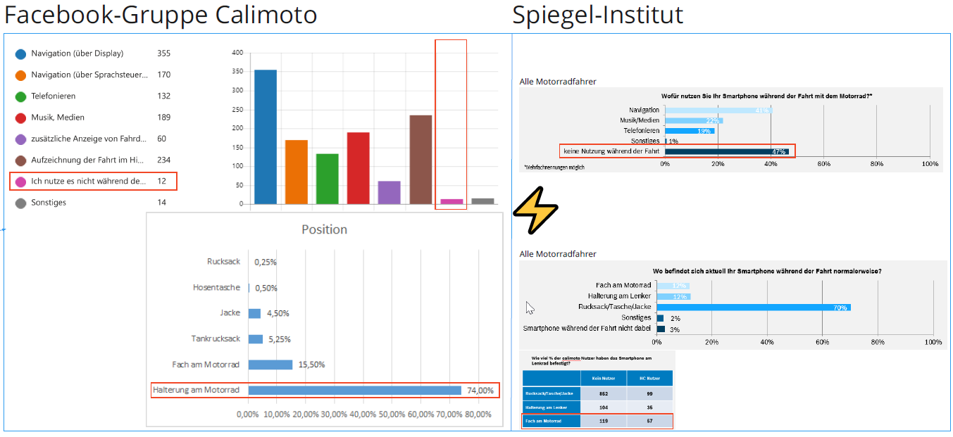
\includegraphics[width=\linewidth]{Bilder/CalimotoUmfragePocketMode.png}
	\caption{Calimoto - Umfrage - Pocketmode}
	\label{fig:CalimotoUmfragePocketMode}
\end{figure}

Aus diesem Grund ist die Entwicklung einer Unfallerkennung im Pocket-Mode wichtig, wo das Smartphone nicht mehr unbedingt am Lenker befestigt werden muss. Die Weiterentwicklung der Unfallerkennung wird mit agilen Methoden erfolgt, \autopageref{abs:MethodenderSoftwareentwicklung}.

\section{Kritische Szenarien/Fälle}
In \autoref{abs:Unfallerkennungsalgorithmus} ist der Ablauf der aktuellen Unfallerkennungsalgorithmus sowie deren Parameter (z.B. TipOver) erläutert. Die Entwicklung des Pocket-Modes sollte auf keinen Fall zu Konflikten mit dem normalen Mode führen. Die aktuelle Zuverlässigkeit des Algorithmus' darf ebenso durch das Pocket-Mode nicht verringert werden, in dem ein im normalen Modus gut erkennbares Unfallszenario durch das Pocket-Mode übersehen wird.
Um die Konflikte zu vermeiden wird eine Liste der Use- sowie Edgecases vorbereitet, in der die Erwarteten Reaktion des aktuellen Algorithmus' aufgelistet wird. Dadurch erfolgt eine Übersicht der möglichen Konflikten sowie der Fällen, wo ein falscher Alarm ausgelöst werden könnte, und gleich eine mögliche Gegenmaßnahme.

%Liste der Edge- und usecases mit einer Erklärung, warum diese kritisch sind und einen Vorschlag, was man dagegen tun kann.
Die \autoref{fig:EdgeCasesExcel} zeigt die erwähnte Liste. Da das Verhalten des Smartphones in der Hosentaschen (am Bein) und am Oberkörper unterschiedlich ist, werden diese separat betrachtet. In der Spalte 'Beschreibung' ist eine nähere Erklärung des Szenarios erläutert. Die Spalte 'Erkennung durch den Algo' berichtet, ob der aktuelle Algorithmus das entsprechende Szenario richtig erkennen wird (IO: In Ordnung, NIO: Nicht In Ordnung). Unter 'Bemerkungen' ist eine weitere Erklärung des erwarteten Ergebnisses beschrieben. Bei den kritischen Szenarien, wo der Algorithmus den Fall nicht richtig erkennen würde, ist eine mögliche Gegenmaßnahme zum Korrigieren der Entscheidung des Algorithmus aufgeschrieben.

\begin{figure}[H]
	\centering
	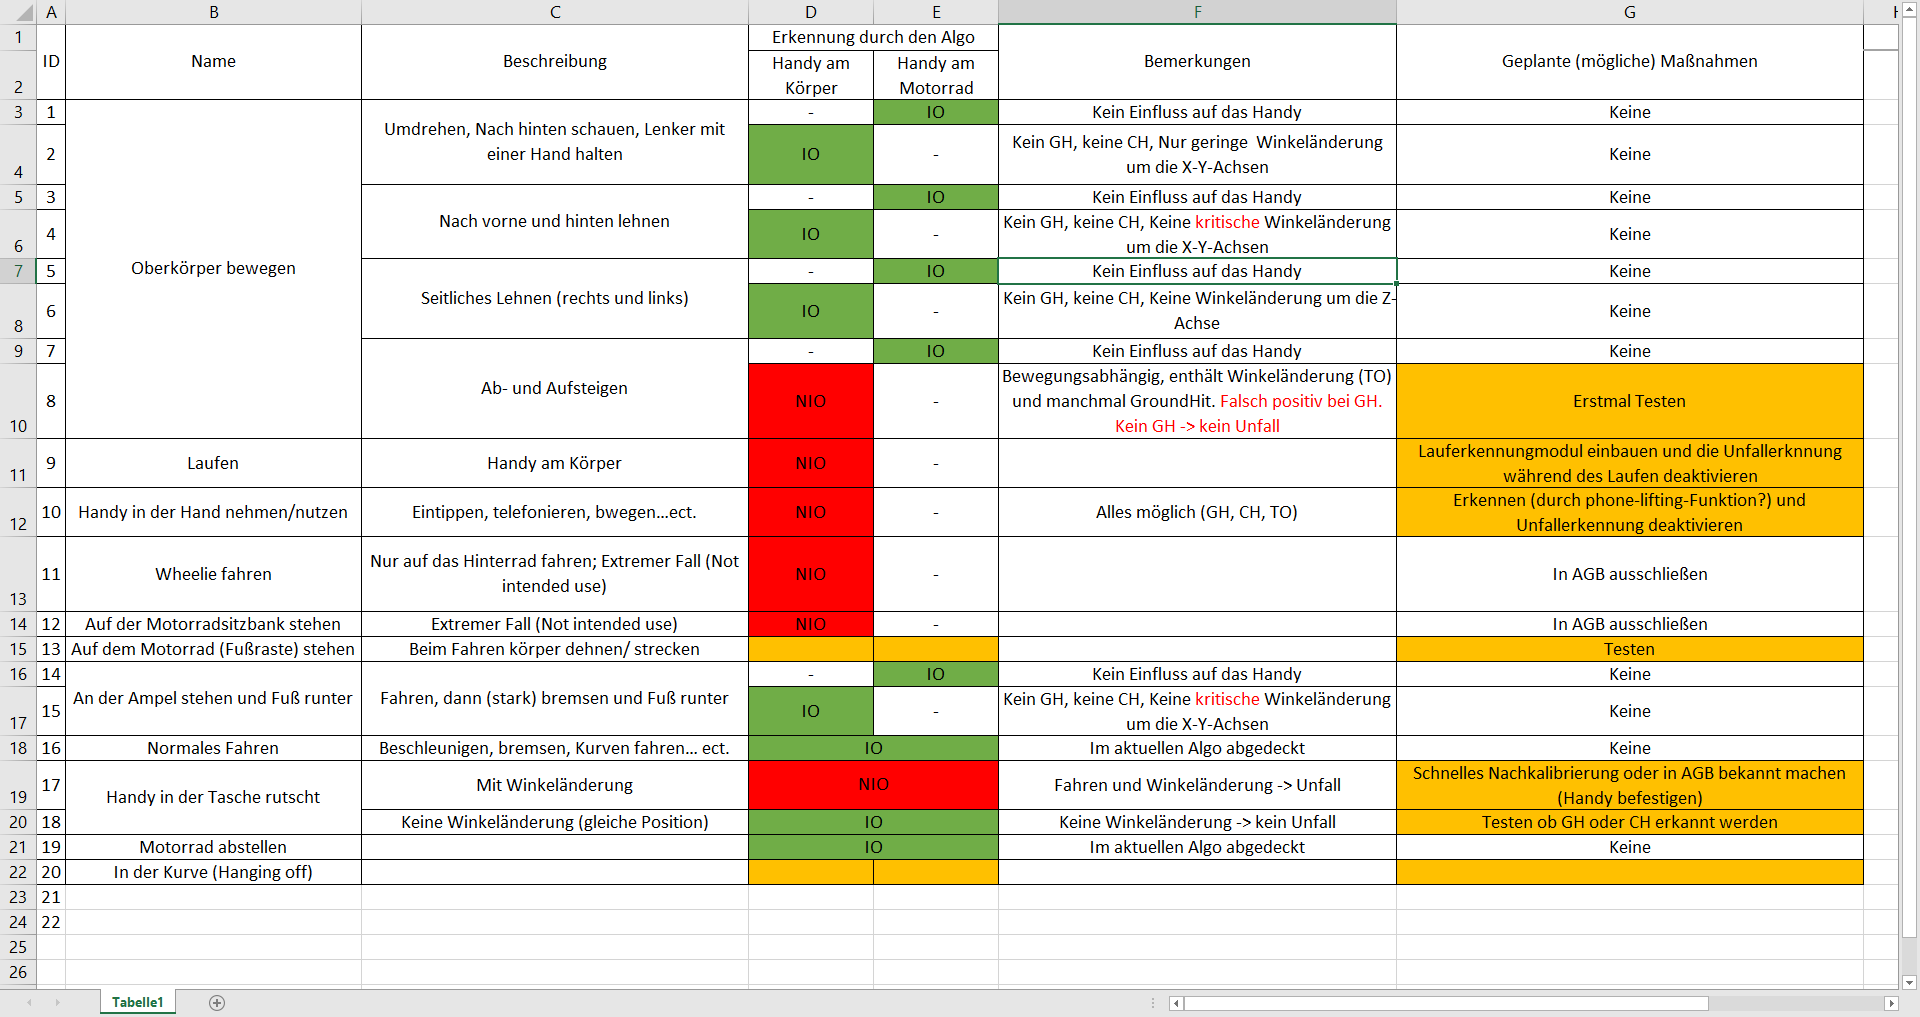
\includegraphics[width=\linewidth]{Bilder/EdgeCasesExcel.png}
	\caption{Liste der Use- und Edgecases mit der erwarteten Reaktion des Algorithmus'}
	\label{fig:EdgeCasesExcel}
\end{figure}

Nach der internen Statistik ist das Laufen ein häufiger Grund von den falschen Alarmen, deswegen eine Lauferkennung zur Verbesserung der Zuverlässigkeit wichtig.

\section{Lauferkennung} \label{sec:Lauferkennung}
In der bereits bestehenden Version des Algorithmus' ist davon ausgegangen, dass das Smartphone am Lenker befestigt wird. Wenn die Person das Handy nach einer Fahrt in die Hosen- bzw. Jackentasche einsteckt und fängt an zu laufen, wird öfters einen falschen Alarm (falsch-positiv) ausgelöst, da das Laufen im bisherigen Algorithmus nicht berücksichtigt wurde.
Wenn die Unfallerkennung im Pocket-Mode verwendet wird, ist stark zu erwarten, dass die Person nach einer Fahrt oder während einer Pause (z.B. Tanken) vergisst (oder ignoriert), die Unfallerkennung zu deaktivieren, und mit dem Smartphone an sich läuft. Das führt dazu, dass die Anzahl der falschen Alarmen im Pocket-Mode wesentlich steigt.

Um diese falsche Auslösungen zu verhindern, ist eine Lauferkennung wichtig. Diese Arbeit beschäftigt sich im Teil mit der Implementierung der Lauferkennung. Das Ziel dahinter ist das Laufen zu erkennen und die Unfallerkennung temporär zu deaktivieren, um die falsche Alarme zu vermeiden und die Agenten zu entlasten.
In diesem Kapital werden die Schritte der Entwicklung der Lauferkennung erläutert.

% Generated using matlabfrag
% Version: v0.6.16
% Version Date: 04-Apr-2010
% Author: Zebb Prime
%
%% <text>
%
\providecommand\matlabtextA{\color[rgb]{0.150,0.150,0.150}\fontsize{11}{11}\selectfont\strut}%
\psfrag{Time}[tc][tc]{\matlabtextA Time}%
%
%% </text>
%
%% <xtick>
%
\def\matlabfragNegXTick{\mathord{\makebox[0pt][r]{$-$}}}
%
\providecommand\matlabtextB{\color[rgb]{0.150,0.150,0.150}\fontsize{10}{10}\selectfont\strut}%
\psfrag{000}[ct][ct]{\matlabtextB $25$}%
\psfrag{001}[ct][ct]{\matlabtextB $30$}%
\psfrag{002}[ct][ct]{\matlabtextB $35$}%
\psfrag{003}[ct][ct]{\matlabtextB $40$}%
\psfrag{004}[ct][ct]{\matlabtextB $45$}%
%
%% </xtick>
%
%% <ytick>
%
\psfrag{005}[rc][rc]{\matlabtextB $-5000$}%
\psfrag{006}[rc][rc]{\matlabtextB $-4000$}%
\psfrag{007}[rc][rc]{\matlabtextB $-3000$}%
\psfrag{008}[rc][rc]{\matlabtextB $-2000$}%
\psfrag{009}[rc][rc]{\matlabtextB $-1000$}%
\psfrag{010}[rc][rc]{\matlabtextB $0$}%
\psfrag{011}[rc][rc]{\matlabtextB $1000$}%
%
%% </ytick>
\begin{figure}[H]
	\centering
	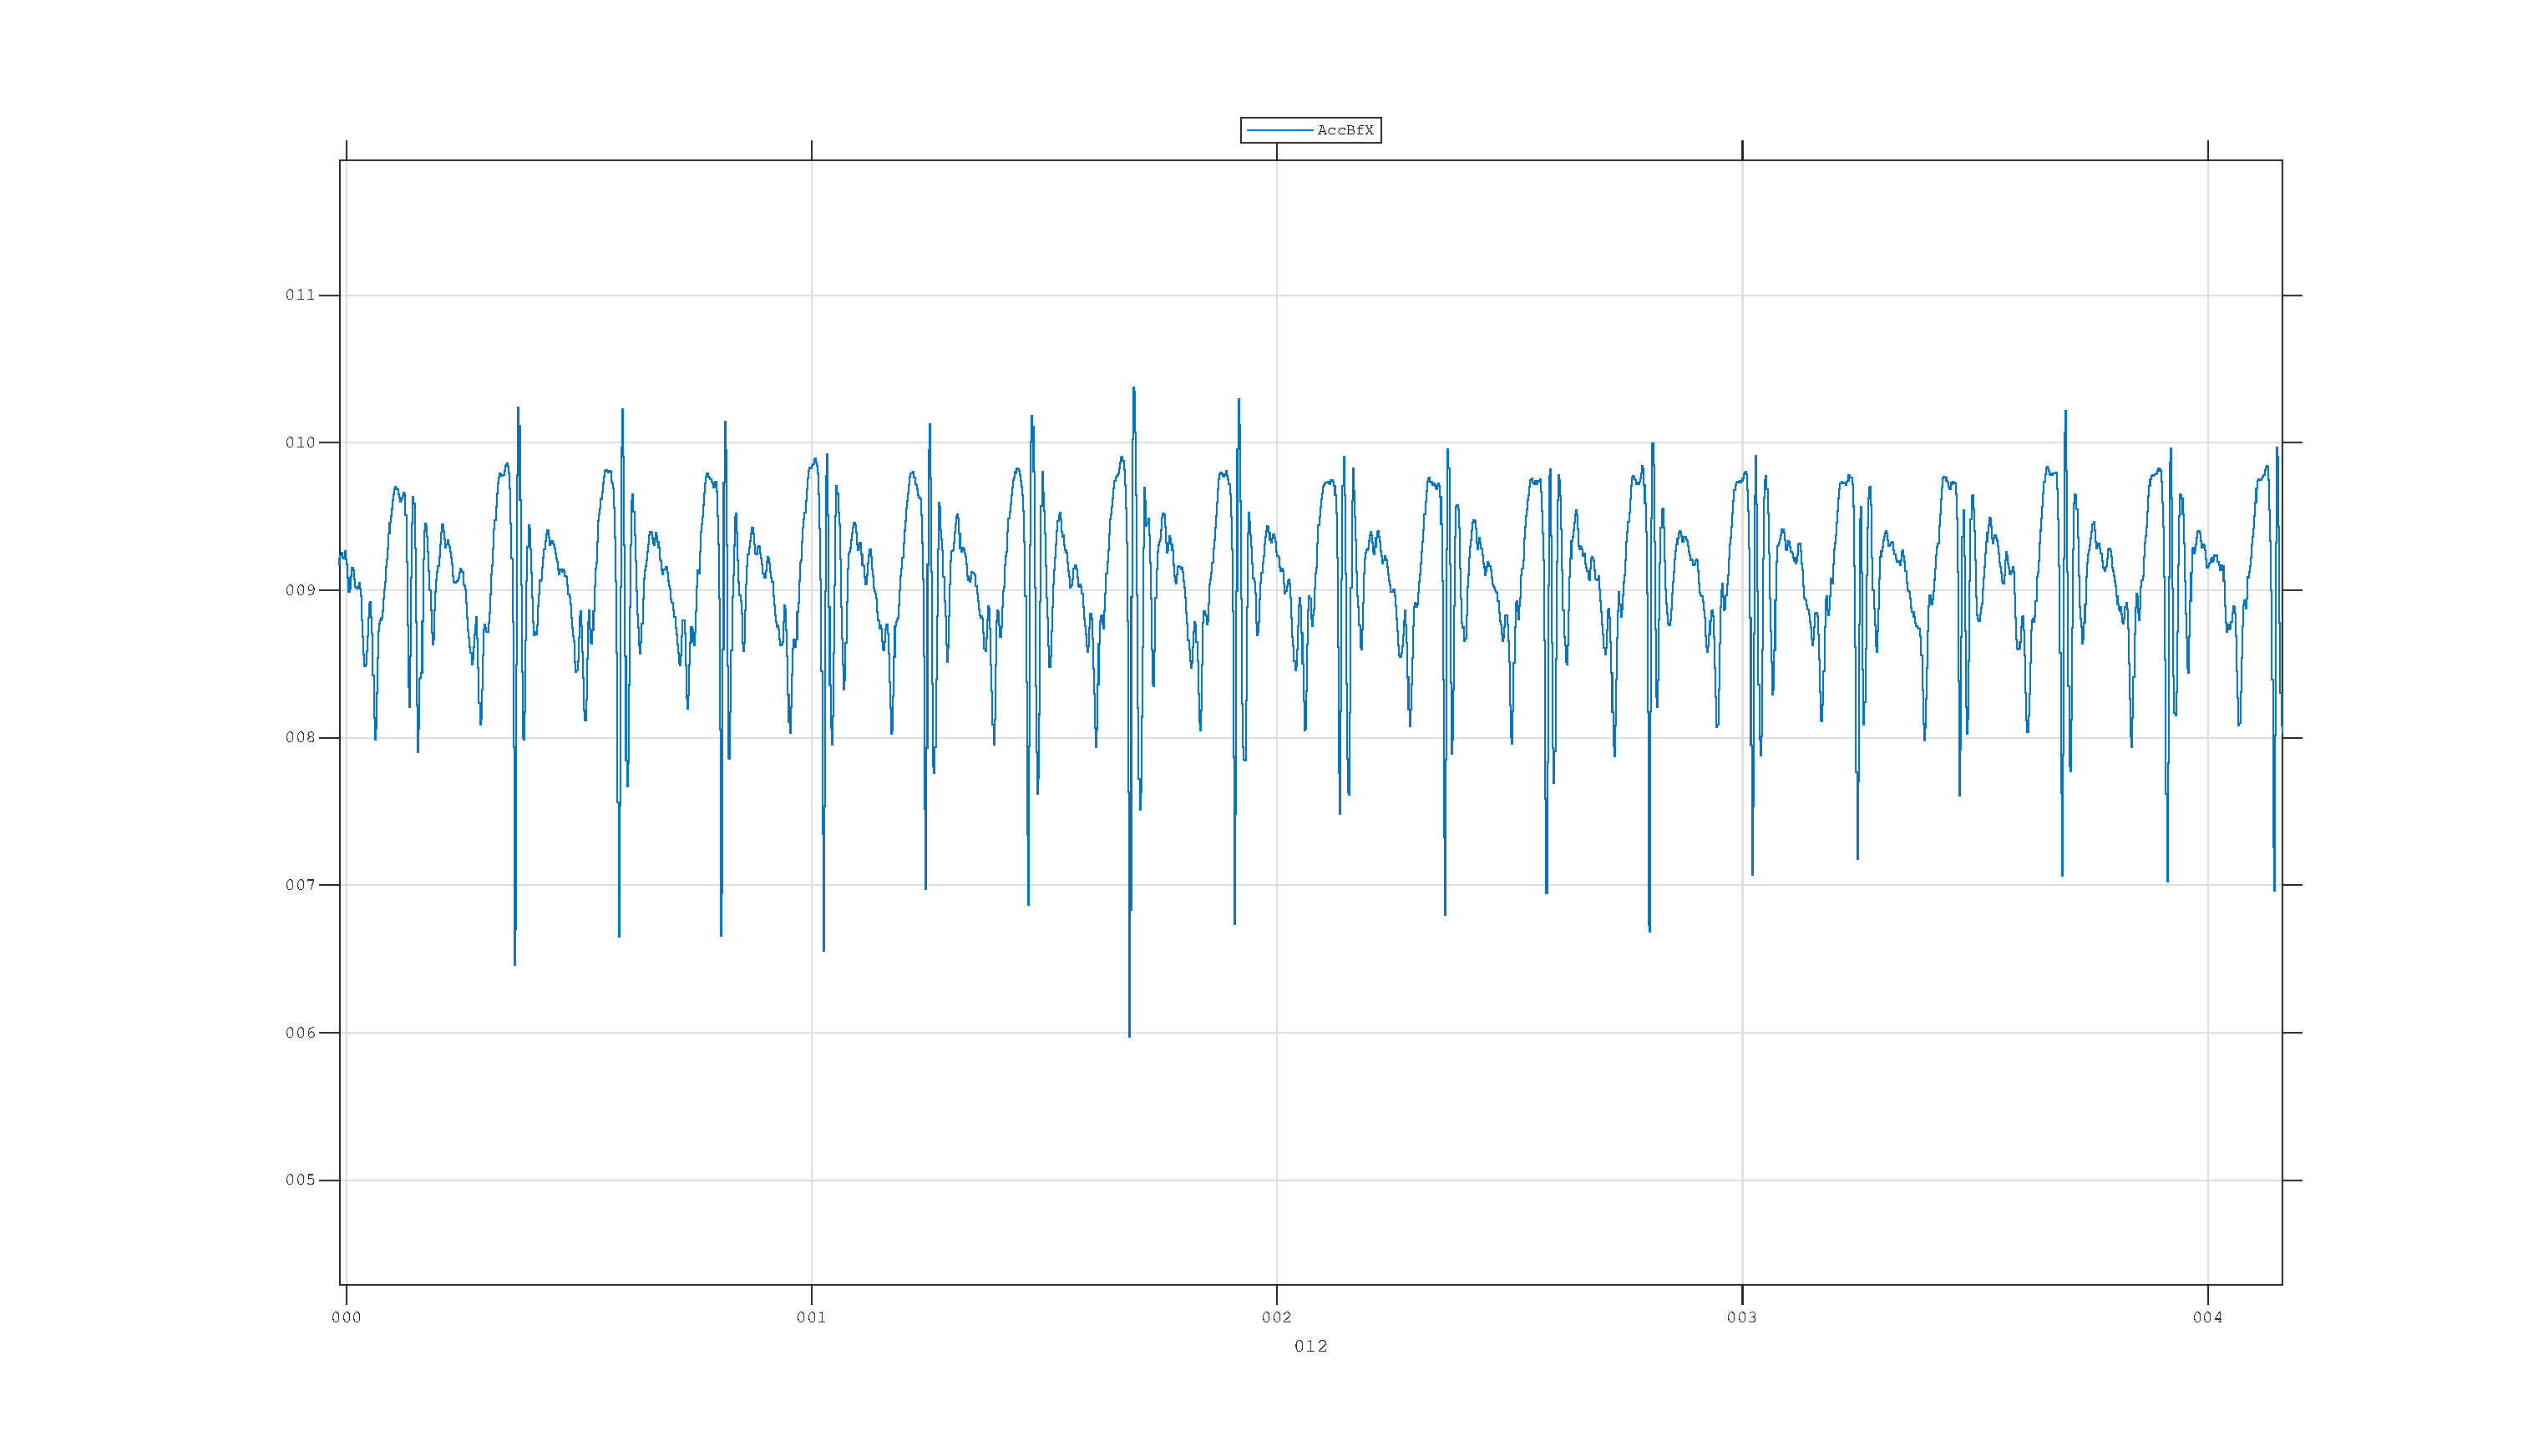
\includegraphics[width=\linewidth]{Bilder/LaufenMuster.eps}
	\caption{Beispiel: Beschleunigungssignal beim Laufen (***x-Achse 0-25 Sekunden, y-Achse (-2500 - 0))}
	\label{fig:LaufenMuster}
\end{figure}
In der \autoref{fig:LaufenMuster} ist ein Beispielsignal aus dem Beschleunigungssensor im Smartphone während des Laufens. Die Person kann bis zu 2 Schritte pro Sekunde im Schnitt zurücklegen. In der Grafik können die Peaks innerhalb einer Sekunde aufgezählt werden und die Anzahl der Schritte ermitteln. Wenn diese unter 2 pro Sekunde sind, ist vom Laufen auszugehen, da ein Motor so wenige Umdrehungen pro Sekunde nicht schafft. Im nächsten Abschnitt werden diese Peaks aufgezählt, um die Anzahl der Schritte bzw. Umdrehungen zu ermitteln.
%
\subsection{Lauferkennung - Spitzendzähler} \label{abs:PeaksAufzaehlen}

Wie bereits erwähnt wurde, kann die Person bis zu vier Schritte pro Sekunde laufen. D.h. aus einem typischen Laufsignal (z.B. \autoref{fig:LaufenMuster}) soll maximal 4 Schritte (zwei Bewegungen pro Fuß) pro Sekunde aufgezählt werden.
Es soll ein Modell implementiert werden, das die Anzahl der Schritten bzw. der Peaks aufzählt und der Mittelwert davon pro Sekunde zurückgibt. Zur Vereinfachung der Implementierung ist eine Testumgebung (siehe. \autoref{fig:Lauferkennung_Peaks_Testbeispiel}) aufgebaut. In der Umgebung wird ein bekanntes Sinussignal generiert und dargestellt.
\begin{figure}[H]
	\centering
	\includegraphics[width=\linewidth]{Bilder/Lauferkennung_Peaks_Testbeispiel.png}
	\caption{Testbeispiel - Lauferkennung - Peaks Zähler}
	\label{fig:Lauferkennung_Peaks_Testbeispiel}
\end{figure}

Die \autoref{fig:Lauferkennung_Peaks_SinusSignalGenerator} zeigt die Spezifikationen des generierten Signals und die \autoref{fig:Lauferkennung_Peaks_SinusSignal} stellt mithilfe eines Scopes (Simulink-Block) das entsprechende Signal grafisch dar sowie wie oft das Signal die Nulllinie überschneidet (blau). Aus der Grafik ist die Anzahl der Peaks einfach zu ermitteln und diese beträgt in diesem Fall 100 Hz umgerechnet.
Eine zeitliche Frequenz wird folgendes berechnet:\\
$Freq_Hz = \frac{Freq_(rad/sec)}{2\pi}$
\begin{figure}[H]
	\centering
	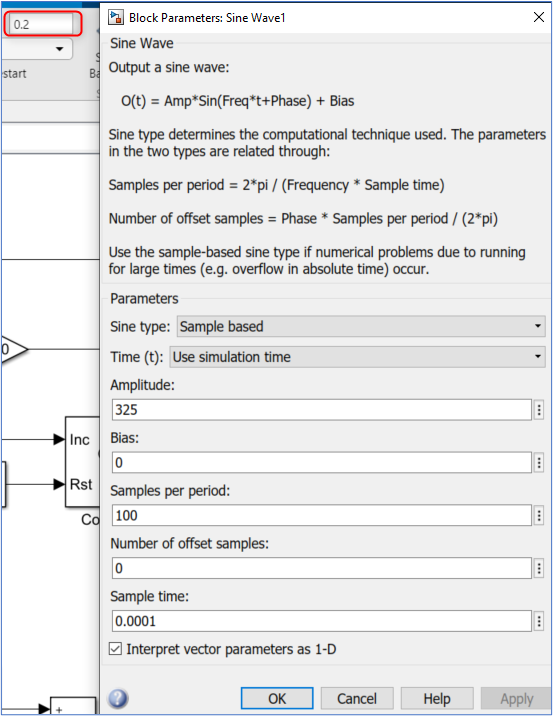
\includegraphics[width=0.5\linewidth]{Bilder/Lauferkennung_Peaks_SinusSignalGenerator.png}
	\caption{Testbeispiel - Lauferkennung - Sinussignalgenerator - Spezifikationen}
	\label{fig:Lauferkennung_Peaks_SinusSignalGenerator}
\end{figure}
\begin{figure}[H]
	\centering
	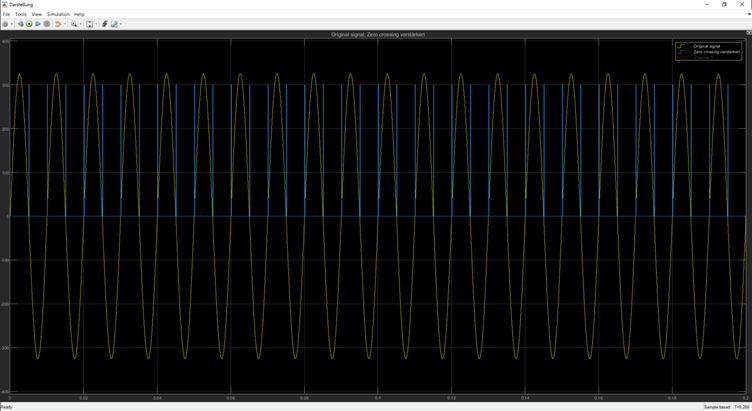
\includegraphics[width=\linewidth]{Bilder/Lauferkennung_Peaks_SinusSignal.png}
	\caption{Testbeispiel - Lauferkennung - Sinussignal}
	\label{fig:Lauferkennung_Peaks_SinusSignal}
\end{figure}
In dem Modell ist die Funktion 'Zero Crossing' verwendet. Diese zählt wie oft das Signal die x-Achse überquert. Diese Methode liefert das richtige erwartete Ergebnis, wenn das Signal um die x-Achse dargestellt ist. Von der anderen Seite hilft diese Funktion nicht, wenn das Signal ein Offset hat, in dem dieses z.B. um die Linie y = 300 (Verschiebung auf der y-Achse), da in diesem Fall das Signal die x-Achse (amplitudenabhängig) nicht mehr schneidet. Das führt dazu, dass das Ergebnis nicht mehr zuverlässig ist.

Eine andere Methode hat sich ergeben, dass die Funktion 'Counter up' in dem Modell verwendet wird. Dieses Block zählt wie oft das Signals in die positive Richtung zeigt. Das neue Implementierung hat ein zuverlässiges Ergebnis im Vergleich zum originalen Modell geliefert.

Beim Einsetzen des gleichen Vorgehens bzw. Modell auf das richtige Laufsignal (\autoref{fig:LaufenMuster}) wird eine Frequenz von ca. $11$ Hz beim Laufen zurückgegeben.

Nach weiteren Auswertungen und Forschungen wird der Grund des Fehlers entdeckt. Es liegt an den Unterschied zwischen dem perfekten generierten Sinussignal und dem echten Laufsignal. Das echte Signal hat im Vergleich zum generierten viele Störungen (Rauschen). Diese lassen sich durch das benannte Modell nicht ausfiltert oder ignorieren, was zu einem falschen Ergebnis führt. Die \autoref{fig:Skizze_IdealUndEchtSignal} stellt ein gutes Beispiel dieser Unterschied dar. Die Rauschen erhöhen die Anzahl der Spitzen.


\begin{figure}[H]
	\centering
	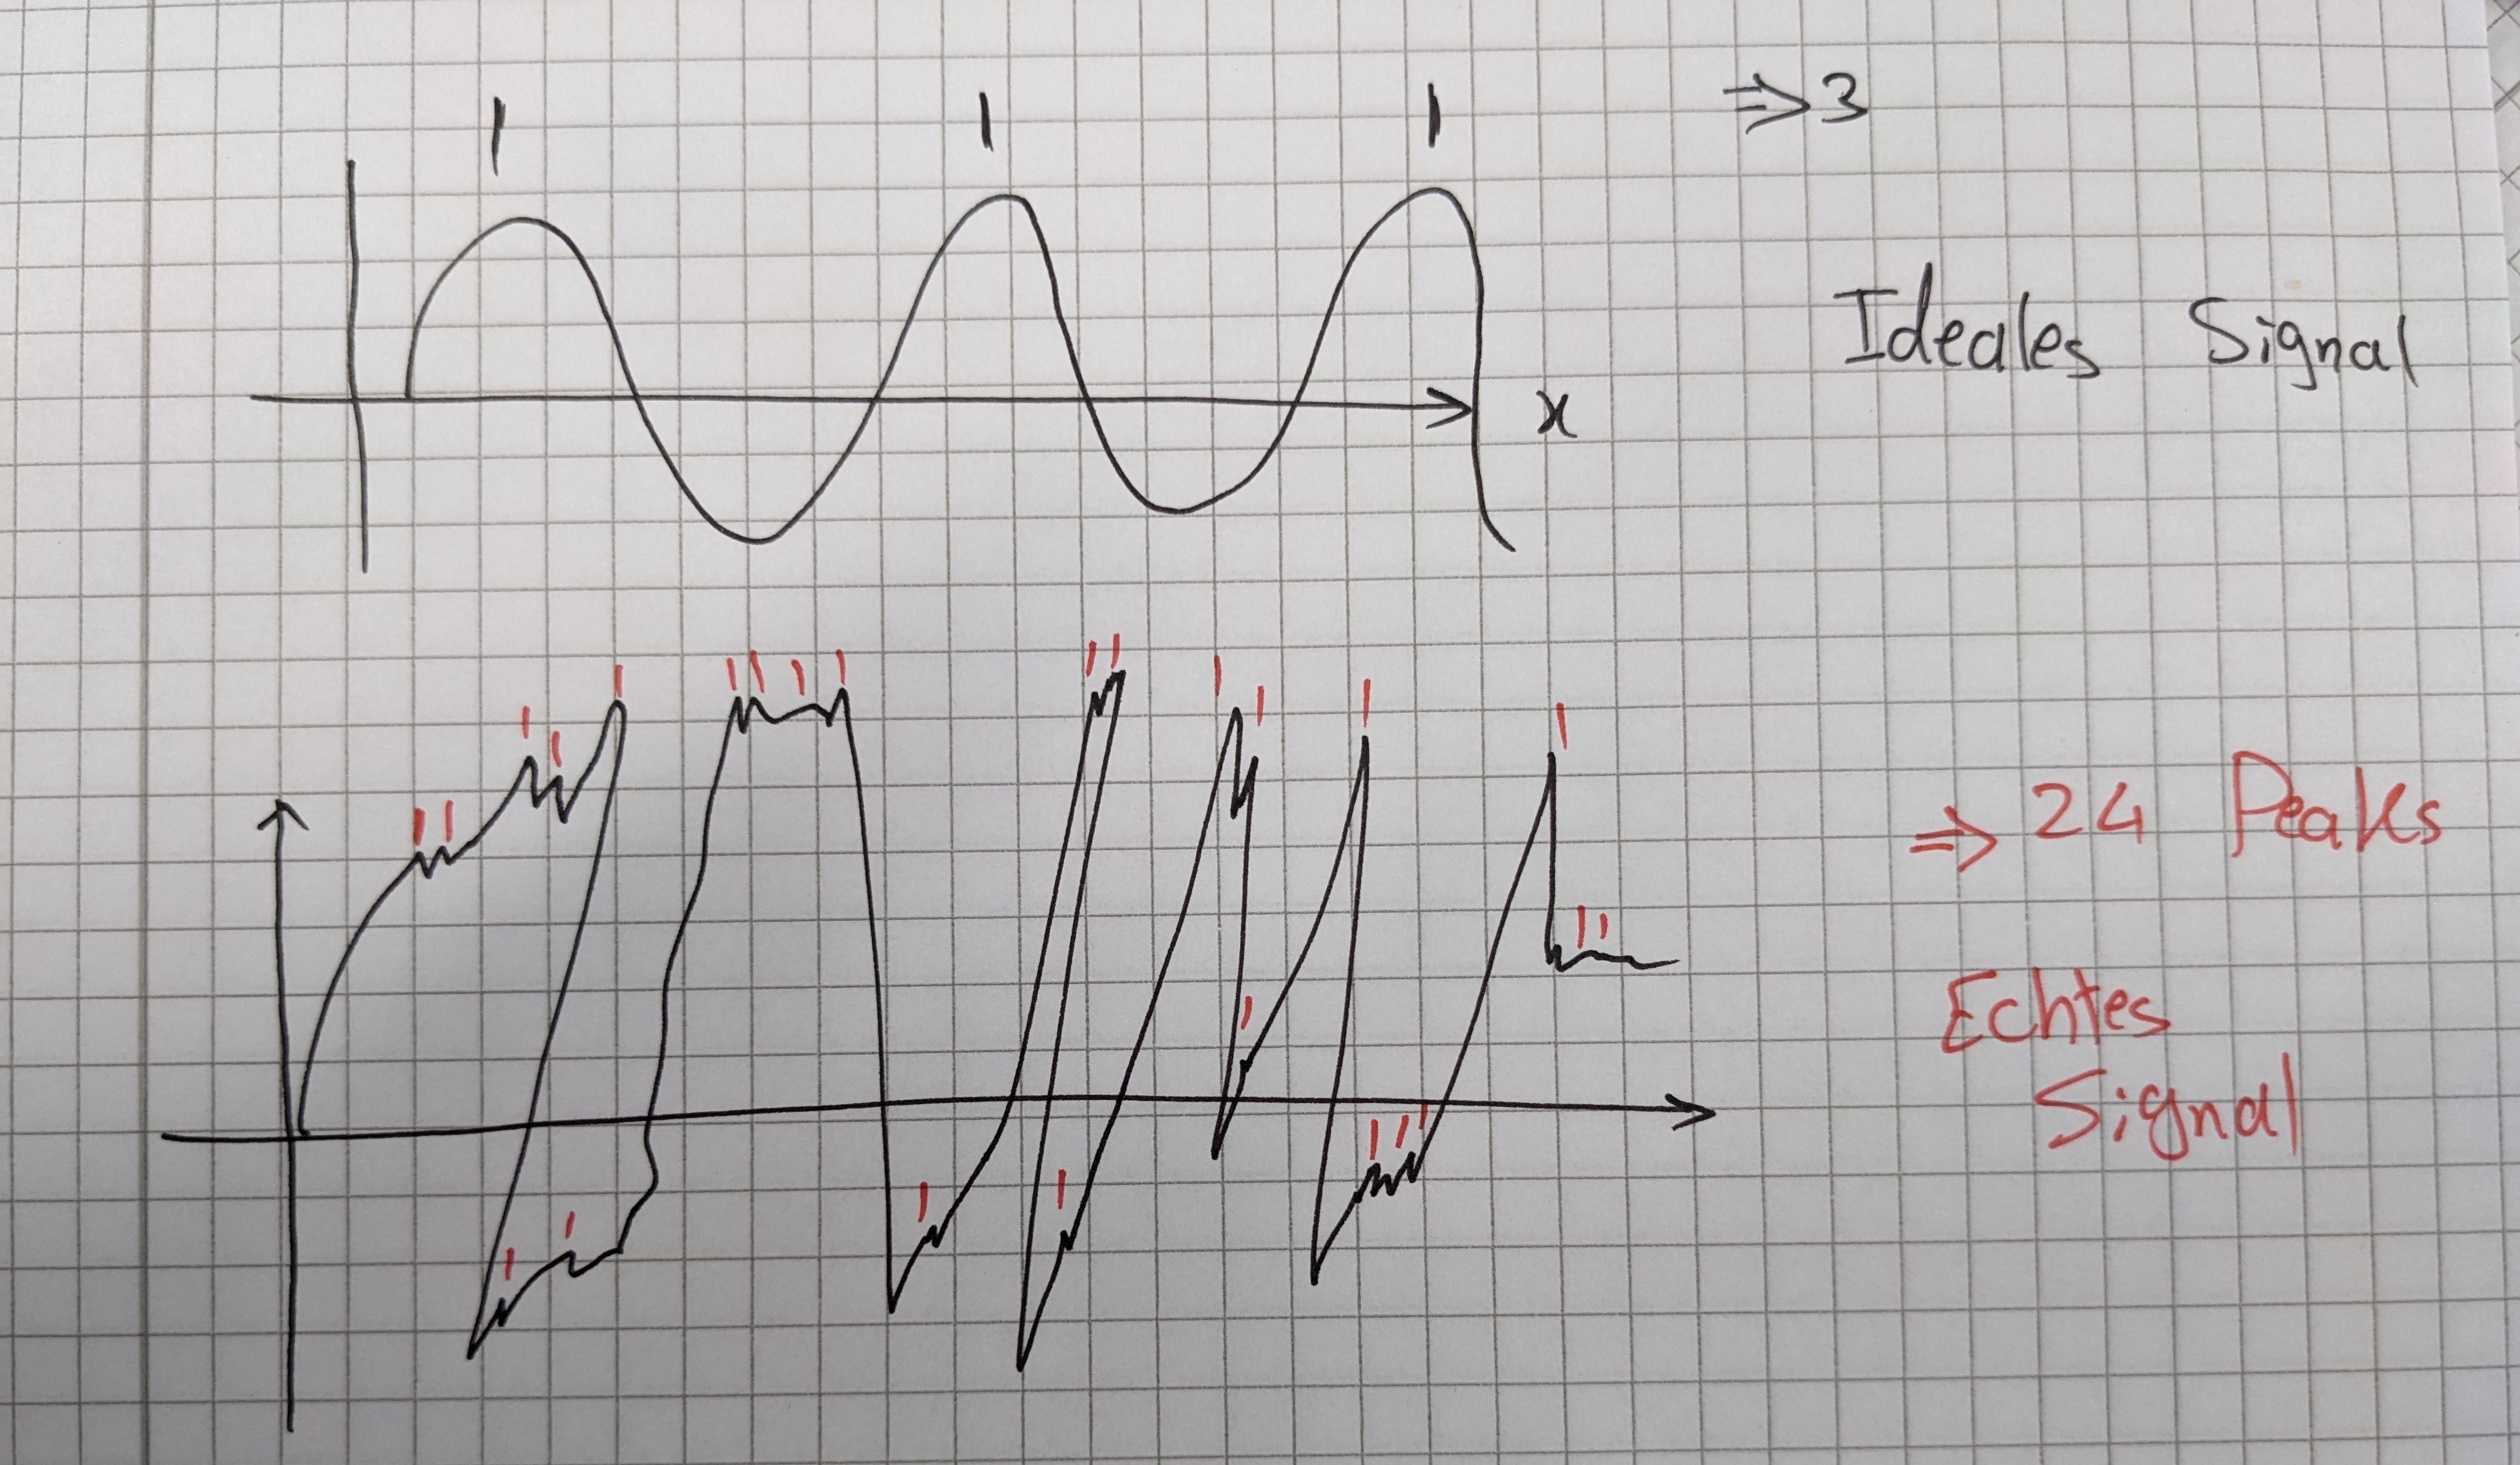
\includegraphics[width=\linewidth]{Bilder/Skizze_IdealUndEchtSignal.jpg}
	\caption{Skizze - Idealsignal und Echtsignal}
	\label{fig:Skizze_IdealUndEchtSignal}
\end{figure}

%Einen Zähler zu implementieren. Das soll alle Peaks aufzählen mit der Hoffnung, dass es Unterschied zwischen Laufen und Fahren zu erkennen ist.
%Das LaufFrequenz ist zwischen 0.5-4 Hz. Das Fahren ist über 20 Hz.
%Es wurde einen Testbeispiel mit einem Sinussignal gebaut und das Prinzip getestet.


%In der \autoref{fig:Lauferkennung_Peaks_Testbeispiel} ist das Beispielmodell zur Lauferkennung basiert auf das Zählen jedes Peak des Signals. Im Modell wurde ein Sinussignal generiert (\autoref{fig:Lauferkennung_Peaks_SinusSignalGenerator}) und dieses bearbeitet und das Prinzip dadurch getestet.

%\autoref{fig:Lauferkennung_Peaks_SinusSignal} zeigt die Ausgabe der Scope-Funktion. In der Grafik ist das generierte Sinussignal (gelb) sowie wie of das Signal die Nulllinie überschneidet (blau).
%In der Scope-Darstellung sind das originale Sinussignal und ein Zähler sichtbar. Der Zähler hat jeden ‚Zero-crossing‘ aufgezählt.
%Das Testmodell hat die richtige (erwartete) Ergebnisse geliefert: 100 Hz als Frequenz.
%Beim Einsetzen des gleichen Vorgehens auf das richtige Signal ($AccBfX_mg$) (das kalibrierten Signal) wurde eine Frequenz von ca. $11$ Hz beim Laufen und eine Frequenz zwischen $20-30$ Hz ausgerechnet. Das hat die Erwartungen nicht entsprochen.
%Daraus kann folgendes extrahiert werden:
%Beide Signale (Szenarien) (Laufen und Fahren) haben die gleiche Menge von Störungen (Rauschen). Der Unterschied ist die Amplitude. Es kann keine Amplitude ‚Hartkodiert‘ entdeckt werden, da die Amplitude sich ständig ändern kann.
%************ Grafiken von den zwei Signalen darstellen und die Art der Rauschen näher analysieren (was könnte die Ursache sein?); Welche mögliche Lösungen gäbe es dafür? *************\\

%\textbf{Ergebnis: Die Frequenz muss allerdings doch gesucht und schließlich verglichen werden}

Da der Spitzenzähler nicht zuverlässig funktioniert, ist eine bessere Idee notwendig. 


\subsection{Frequenzbasierte Lauferkennung} %TODO: ausführlich beschreiben

Das Laufsignal stellt ein wiederholtes Pattern dar, was auch durch die Frequenz erkannt wird.
Das Modell muss diese Frequenz ermitteln und auswerten.
Analog zum \autoref{abs:PeaksAufzaehlen} wird hier nochmal eine neue Hypothese festgelegt, die durch einem Testmodell überprüft werden soll.

Die Hypothese: Die Frequenz während des Laufens sollte kleiner als $2 Hz$ sein und beim Fahren über $7 Hz$. Wenn eine Frequenz von über $7$ Hz ermittelt wird, ist eine Laufaktivität ausgeschlossen, da ein Mensch auf keinen Fall 14 Schritte zurücklegen kann. Die Transformation vom Zeitbereich zum Frequenzbereich wird durch eine FFT erfolgt.

Die Calimoto-App hat eine Abtastrate $f_s = 100$ Hz. D.h. es gibt 100 Messwerte pro Messsekunde.

Bezogen auf die Nyquist-Frequenz (\autoref{gl:Nyquist-Frequenz})ist die Bandbreite bzw. die minimale erkennbare Frequenz $f_n = 50$ Hz.

\subsubsection{Spectrum Analyzer}
In der \autoref{fig:Lauferkennung_Freqbasiert_TestBeispiel_SinussignalGenerator} ist das generierte Sinussignal mit einer Frequenz von $100$ Hz sowie seine Spezifikationen zu sehen.
Es wird in diesem Modell ein Block 'Spectrum Analyzer' (rot markiert) als Referenz verwendet, was die einzelne Frequenzen eines komplexen Signals zurückgibt. Der Benutzer kann die Spezifikationen des 'Spectrum Analyzer's einstellen. Die Ausgabe des Spectrum Analyzers ist in der \autoref{fig:Lauferkennung_Freqbasiert_SpektrumAnalyzerAusgabe} zu sehen. In der Oberen Grafik werden die Intensität der Frequenz(en) (Spektrum genannt) abgebildet und in der unteren Grafik eine 3-D-Darstellung (Frequenz-Zeit-Intensität) (genannt Spektrogramm), wobei die Farbe die Intensität repräsentiert. Wenn die Abbildung näher betrachtet wird, ist eine Frequenz von $100$ Hz gut sichtbar.

\begin{figure}[H]
	\centering
	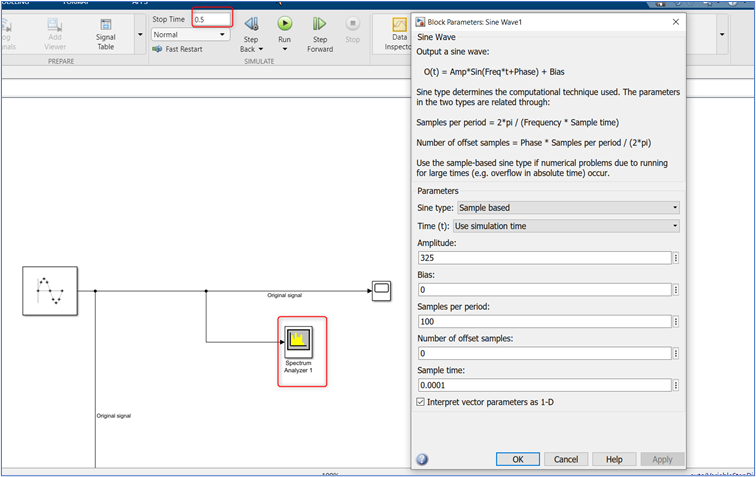
\includegraphics[width=\linewidth]{Bilder/Lauferkennung_Freqbasiert_TestBeispiel_SinussignalGenerator.png}
	\caption{Testbeispiel - Frequenzbasierte Lauferkennung - Sinussignal}
	\label{fig:Lauferkennung_Freqbasiert_TestBeispiel_SinussignalGenerator}
\end{figure}

\begin{figure}[H]
	\centering
	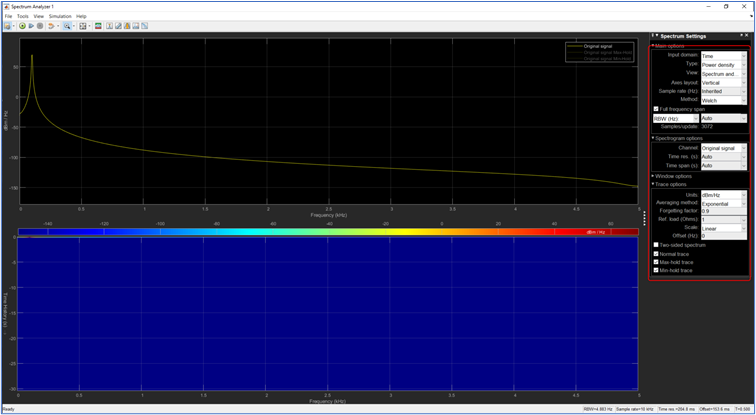
\includegraphics[width=\linewidth]{Bilder/Lauferkennung_Freqbasiert_SpektrumAnalyzerAusgabe.png}
	\caption{Testbeispiel - Frequenzbasierte Lauferkennung - Ausgabe des Spektrum-Analyzer und seine Spezifikationen}
	\label{fig:Lauferkennung_Freqbasiert_SpektrumAnalyzerAusgabe}
\end{figure}

\begin{figure}[H]
	\centering
	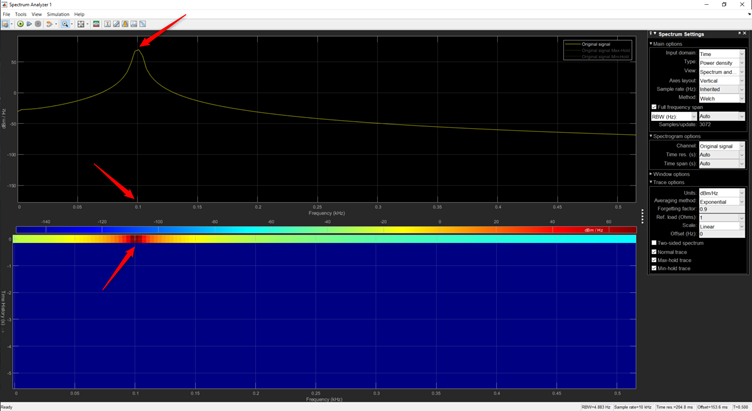
\includegraphics[width=\linewidth]{Bilder/Lauferkennung_Freqbasiert_SpektrumAnalyzerAusgabe_gezoomt.png}
	\caption{Testbeispiel - frequenzbasierte Lauferkennung - Ausgabe des Spektrum-Analyzer im Bereich zwischen 0-0.5 kHz}
	\label{fig:Lauferkennung_Freqbasiert_SpektrumAnalyzerAusgabe_gezoomt}
\end{figure}

Mit anderen Einstellungen in dem Spektrum-Analyzer erhält der Benutzer eine aussagekräftigere Darstellung der Frequenz (siehe \autoref{fig:Lauferkennung_Freqbasiert_SpektrumAnalyzerAusgabe_2Einstellungen})

\begin{figure}[H]
	\centering
	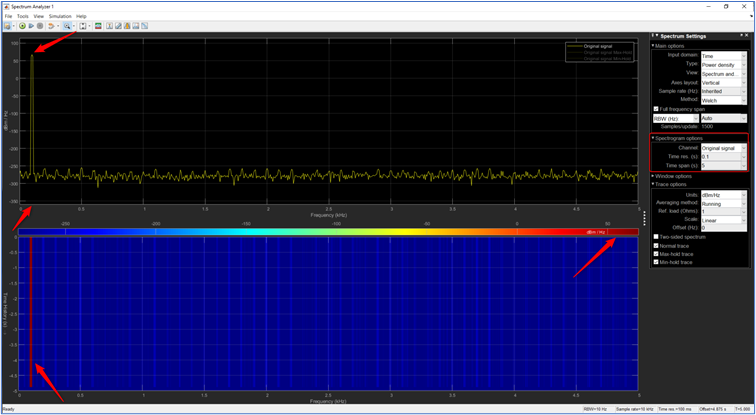
\includegraphics[width=\linewidth]{Bilder/Lauferkennung_Freqbasiert_SpektrumAnalyzerAusgabe_2Einstellungen.png}
	\caption{Testbeispiel - Frequenzbasierte Lauferkennung - Ausgabe des Spektrum-Analyzer mit anderen Spezifikationen}
	\label{fig:Lauferkennung_Freqbasiert_SpektrumAnalyzerAusgabe_2Einstellungen}
\end{figure}

\subsubsection{Testmodell}
Ein Testmodell ist in der \autoref{fig:Lauferkennung_Freqbasiert_FFT_Testmodell} abgebildet. Das Ziel ist die Funktionalität des Prinzips zu überprüfen, bevor dieses mit einem Echtsignal verwendet wird.\\
In dem Modell sind drei Sinussignale mit verschiedenen Frequenzen generiert, die zusammen summiert werden, um ein komplexes Signal zu erstellen.
Die drei Sinussignale sowie deren Summe sind in der \autoref{fig:Testsignal_AllViews} dargestellt.

Das Testmodell erstellt zuerst ein komplexes Signal mit bekannten Einzel- bzw. Grundfrequenzen und konvertiert dieses zu einem diskreten Signals, da die FFT nicht auf ein kontinuierliches Signal anwendbar. Danach wird das FFT-Fenster durch das 'Buffer'-Block ermittelt und dann eine FFT für das entsprechende Fenster verwendet. Das Ergebnis der FFT wird weiterbearbeitet, in dem der Betrag gebildet und Spiegelung entfernt wird. Das Resultat ist eine 2-D-Matrix, wobei die x-Werte die Frequenzen auf einer Skala von 1-512 und die y-Werte die Intensität jeder Frequenz sind. Das Resultat ist in der \autoref{fig:FFT_Ergebnis_Skala_512} dargestellt. Die X-Werte (bzw. Indexe) werden extrahiert und in den Skala von 1-100 umgerechnet, in dem diese mit $100/512$ multipliziert. Eine vereinfachte Ablaufschema ist in der \autoref{fig:Lauferkennung_FFT_Ablaufschema_Testmodell} abgebildet.
Das Endergebnis des Modells ist eine sortierte Liste von den tatsächliche Frequenzen. Die ersten drei Werte haben eine wesentliche große Intensität und sind somit die gesuchten Frequenzen mit kleiner Abweichung.

\begin{landscape}
	\begin{figure}[H]
		\centering
		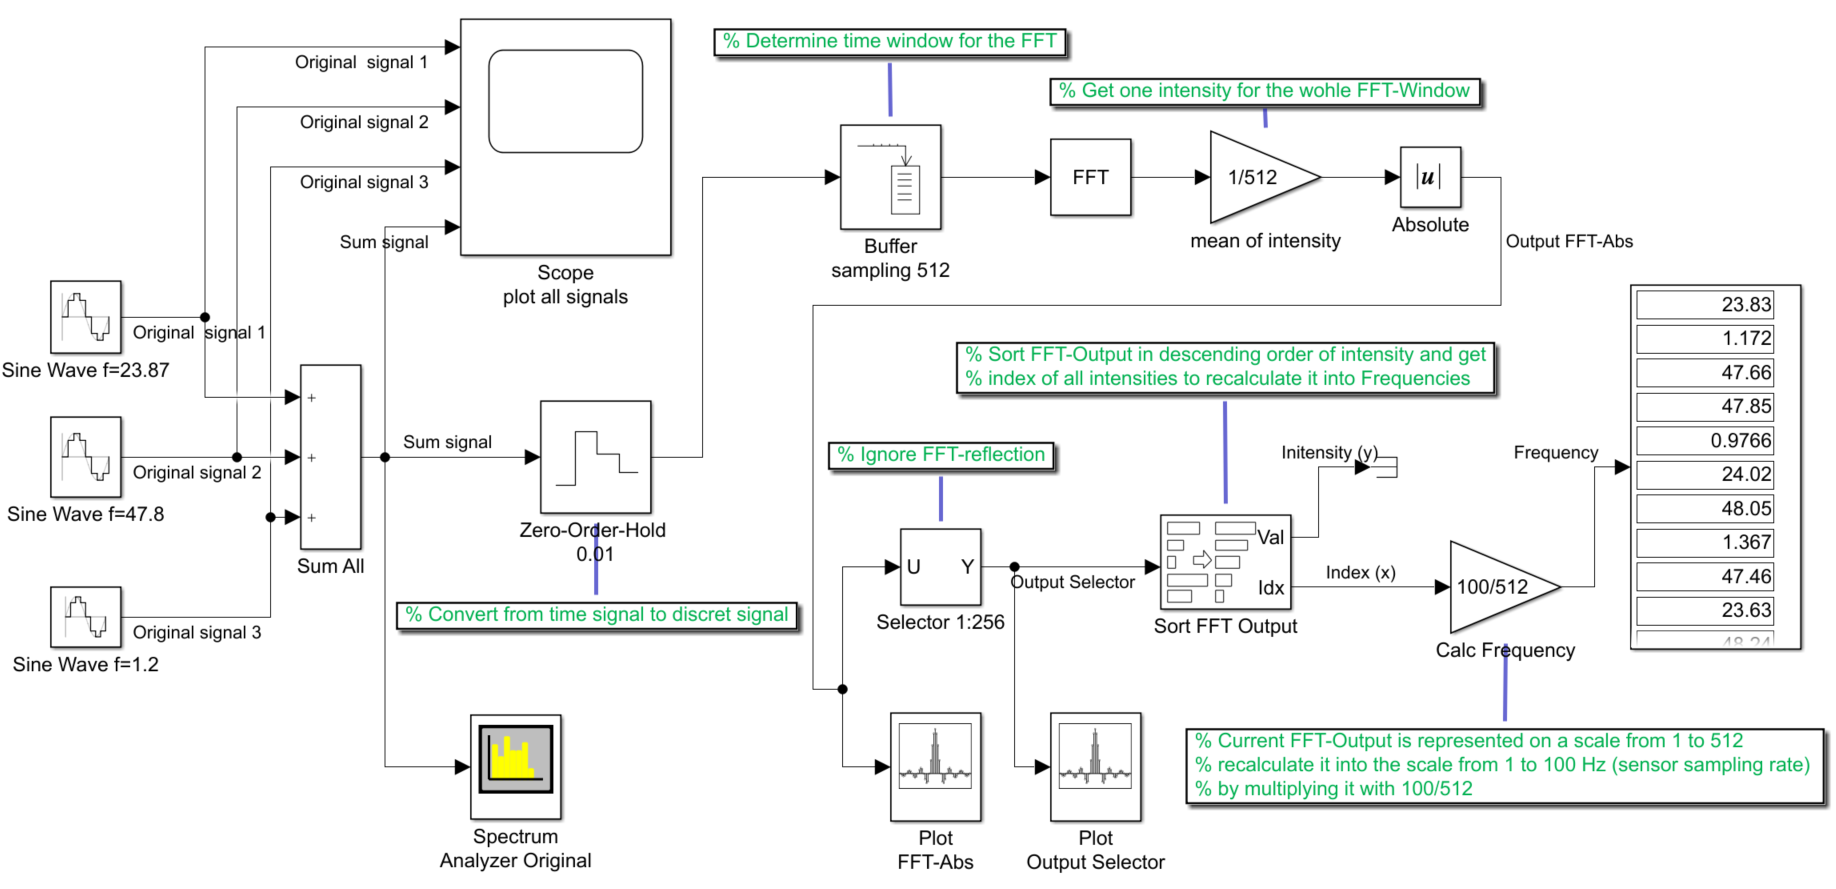
\includegraphics[width=\linewidth]{Bilder/Lauferkennung_FFT_Testmodell1.png}
		\caption{Testbeispiel - Frequenzbasierte Lauferkennung - FFT}
		\label{fig:Lauferkennung_Freqbasiert_FFT_Testmodell}
	\end{figure}
\end{landscape}

\begin{figure}[H]
	\centering
	\includegraphics[width=\linewidth]{Bilder/Lauferkennung_FFT_Ablaufschema_Testmodell.jpg}
	\caption{Ablaufschema des Testmodells}
	\label{fig:Lauferkennung_FFT_Ablaufschema_Testmodell}
\end{figure}

\begin{figure}[H]
	\centering
	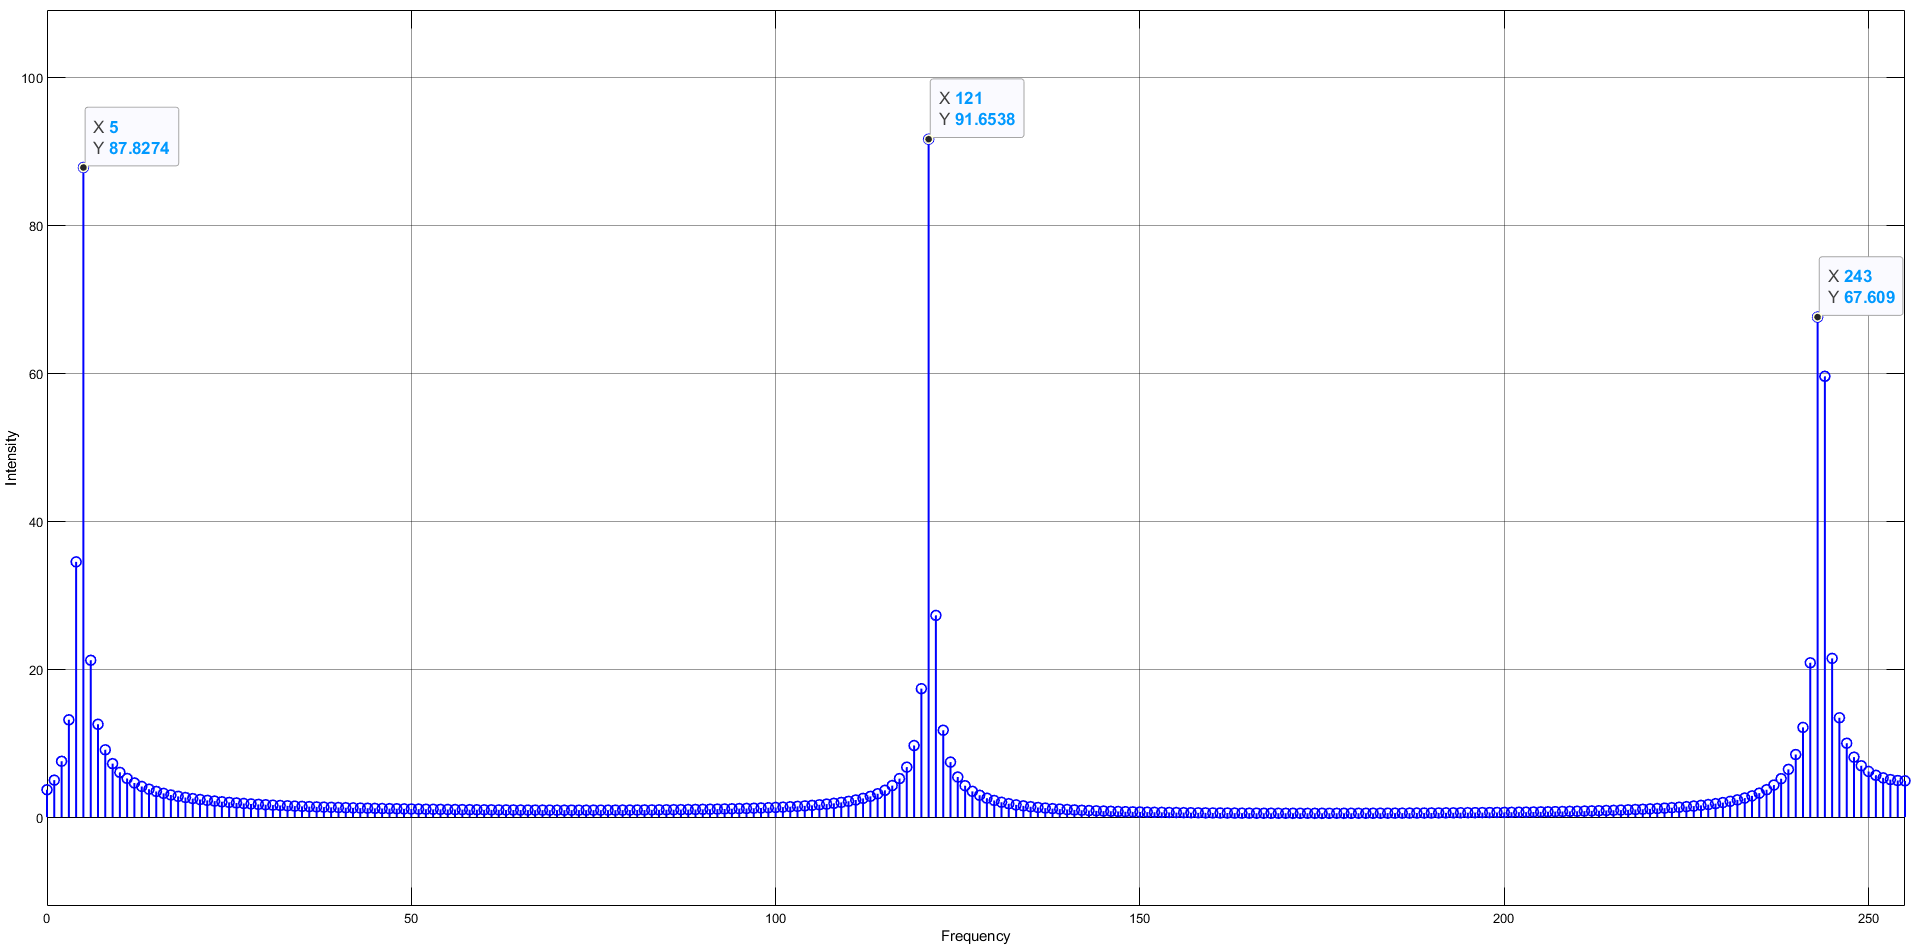
\includegraphics[width=\linewidth]{Bilder/FFT_Ergebnis_Skala_512.png}
	\caption{Das Ergebnis der FFT - Spiegelung entfernt und Beträge}
	\label{fig:FFT_Ergebnis_Skala_512}
\end{figure}
\begin{figure}[H]
	\centering
	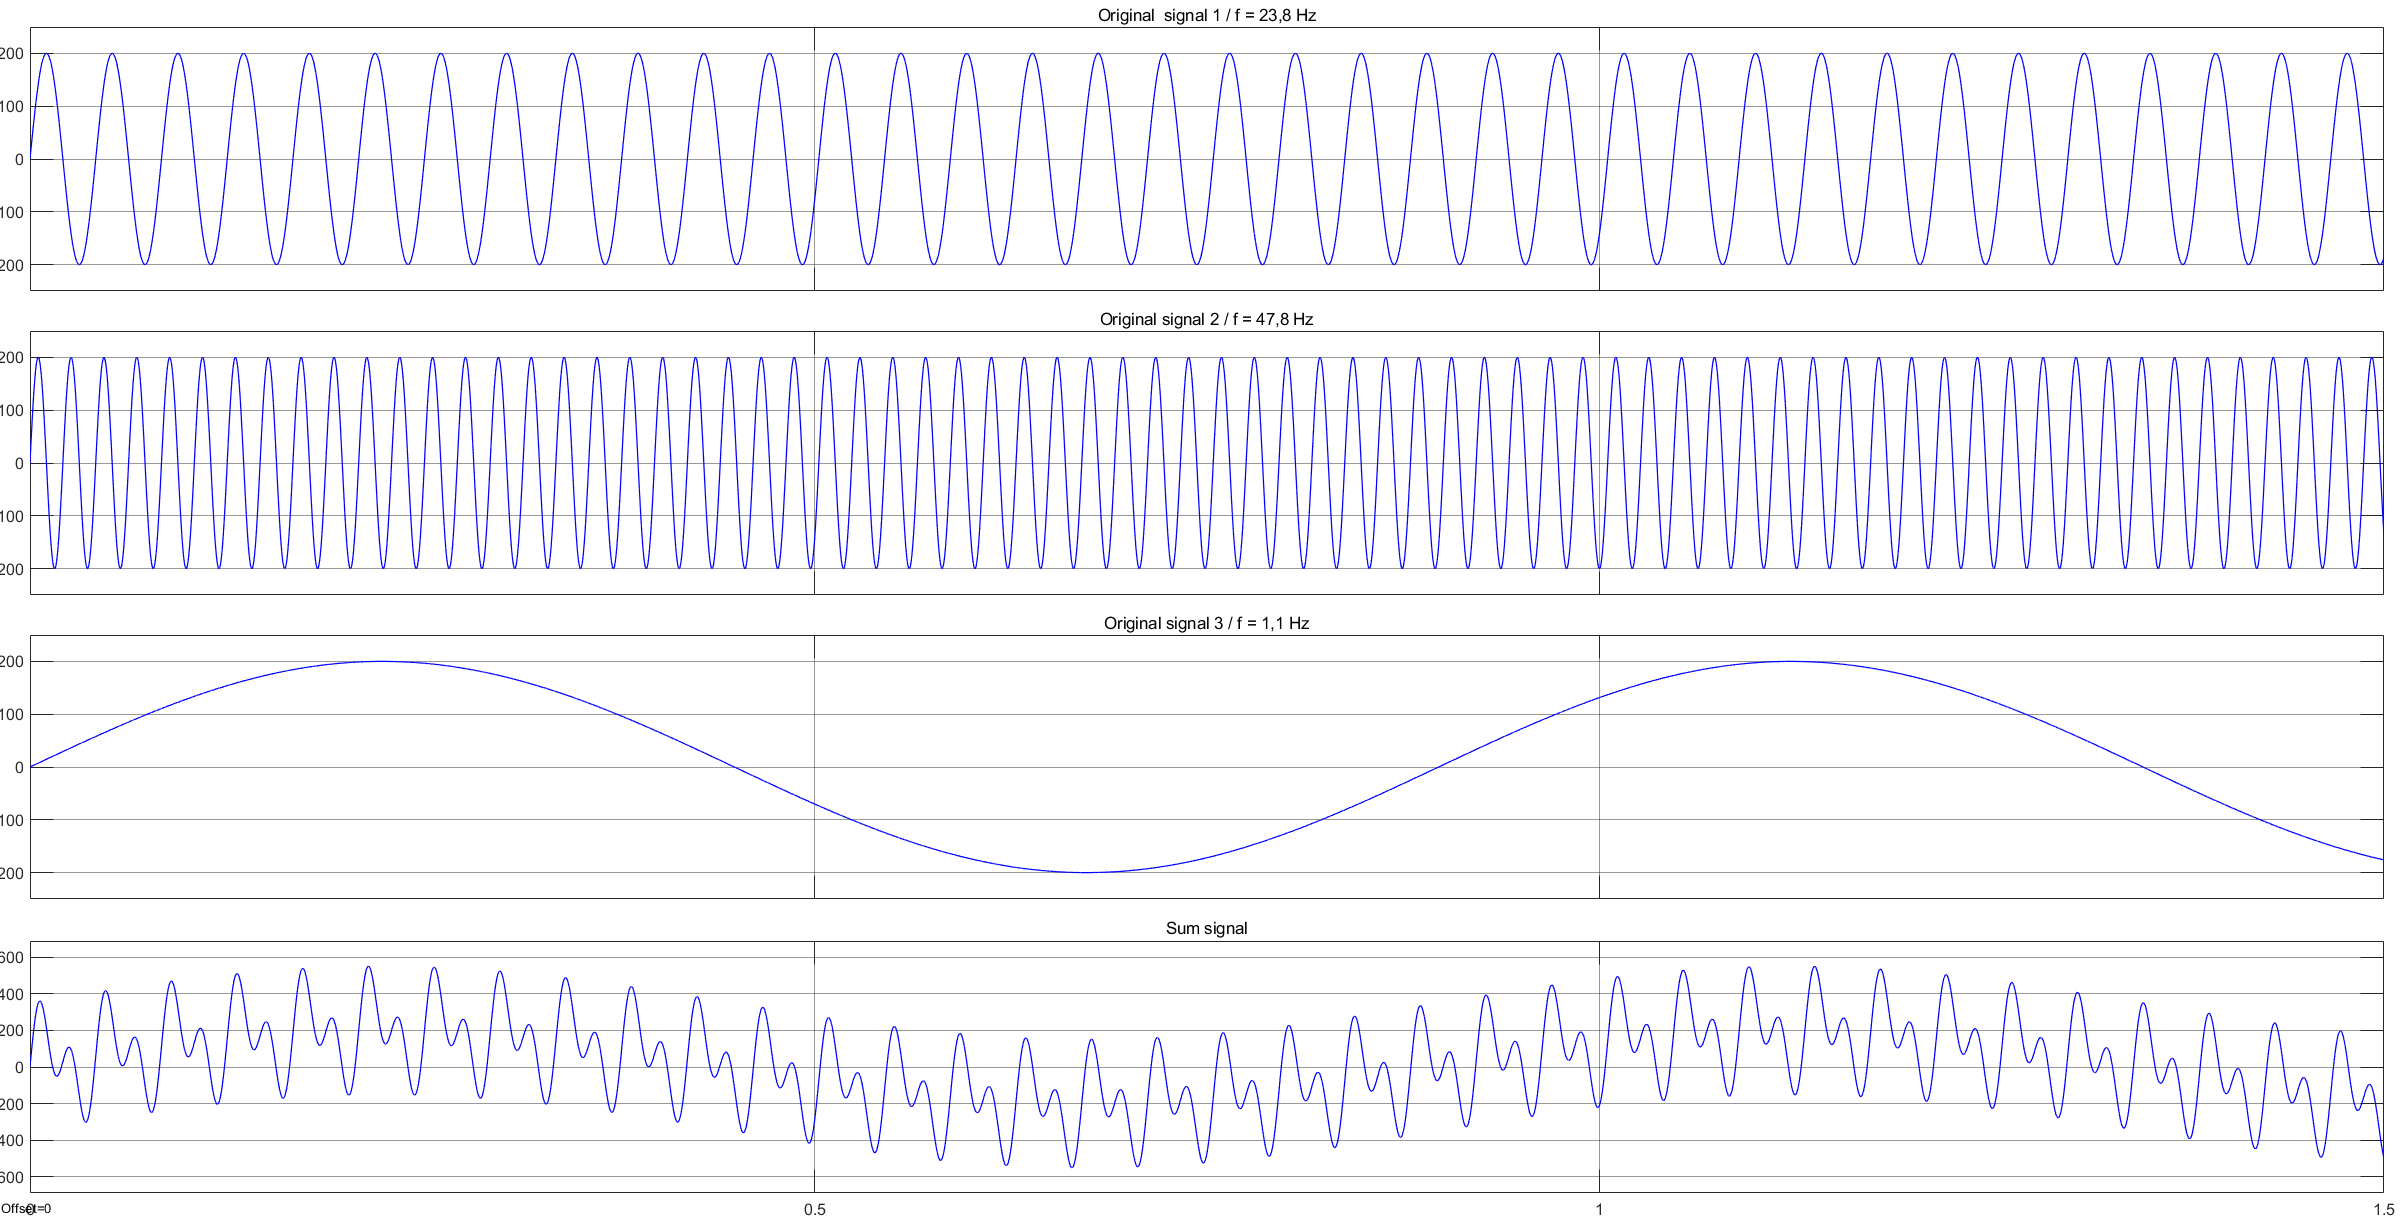
\includegraphics[width=\linewidth]{Bilder/Testsignal_AllViews.png}
	\caption{verschiedene Signale ($f=23,8$; $f=47,8$; $f=1,1$) mit deren Summe $f_g$}
	\label{fig:Testsignal_AllViews}
\end{figure}

Nachdem die Ergebnisse des Testmodells für Richtigkeit geprüft wurde, wird das Modell mit einem Echtsignal getestet. 

\subsubsection{Anwendung auf ein Echtsignal}

Zum Anwenden auf ein Echtsignal wird ein Untermodell 'MotionDetection' erstellt, das die Bewegung (Laufen oder fahren) erkennt und zurückgibt.
In der \autoref{fig:Lauferkennung_Freqbasiert_FFT_Echtmodell} ist einen Teil des genannten Modells sichtbar. 

Im ersten Teil wird der Betrag aller drei Komponenten der Beschleunigung (X,Y,Z) ausgerechnet und dieser für die Lauferkennung verwendet, um diese unabhängig von der Laufrichtung zu bewahren. Der erste Teil kann wie folgt mathematisch beschrieben werden:
\begin{align*}
	Acc_g = \sqrt{ Acc_X^2 + Acc_Y^2 + Acc_Z^2}
\end{align*}

In dem zweiten Teil wird eine FFT durchgeführt, um danach die Frequenzen ermitteln zu können. Das Block 'Buffer' stellt das FFT-Fenster ($B_L$) ein, in dem die Anzahl der Proben (Messungen) gesammelt werden. In diesem Modell wurde das Fenster auf $B_L = 2,56$ Sekunden (d.h. 256 Proben) mit einer Überlappung von $50\%$ eingestellt. Die minimale erkennbare Frequenz lässt sich durch $f_{min} = \frac{1}{B_L} = 0,3906$ Hz berechnen (siehe \autoref{abs:FFT}).

Eine größeres FFT-Fenster $B_L$ hätte eine bessere Frequenzermittlung gesichert und würde allerdings zu größeren Rechenaufwand und längeren Rechenzeiten führen. Die Überlappung dient dazu die Frequenzen am FFT-Fensterrand besser zu berücksichtigen. Danach wird die FFT-Spiegelung mit der Funktion 'Select' vernachlässigt. Der Ausgang dieses Teils ist eine 2D-Liste auf ein Skala von 1 bis 256, die sortiert werden soll.

Der dritte Teil sortiert die entsprechende Liste nach Intensität. Das Block 'Sort FFT Output' ergibt die Sortierten Intensitäten sowie deren Index in dem ursprünglichen Matrix. Diese Indexe entsprechen die gesuchten Frequenzen auf die originale Skala (1-256). Mit einer Umrechnung in die Skala (1-100) lassen sich die tatsächliche Frequenzen berechnen. Die 'Select'-Blöcke dienen dazu eine Rechenzeit zu verkürzen, in dem nur die ersten zehn Frequenzen (bzw. die Frequenzen mit den größten Intensitäten) ausgesucht werden, da nur diese für die Entscheidung später relevant sind.

\begin{figure}[H]
	\centering
	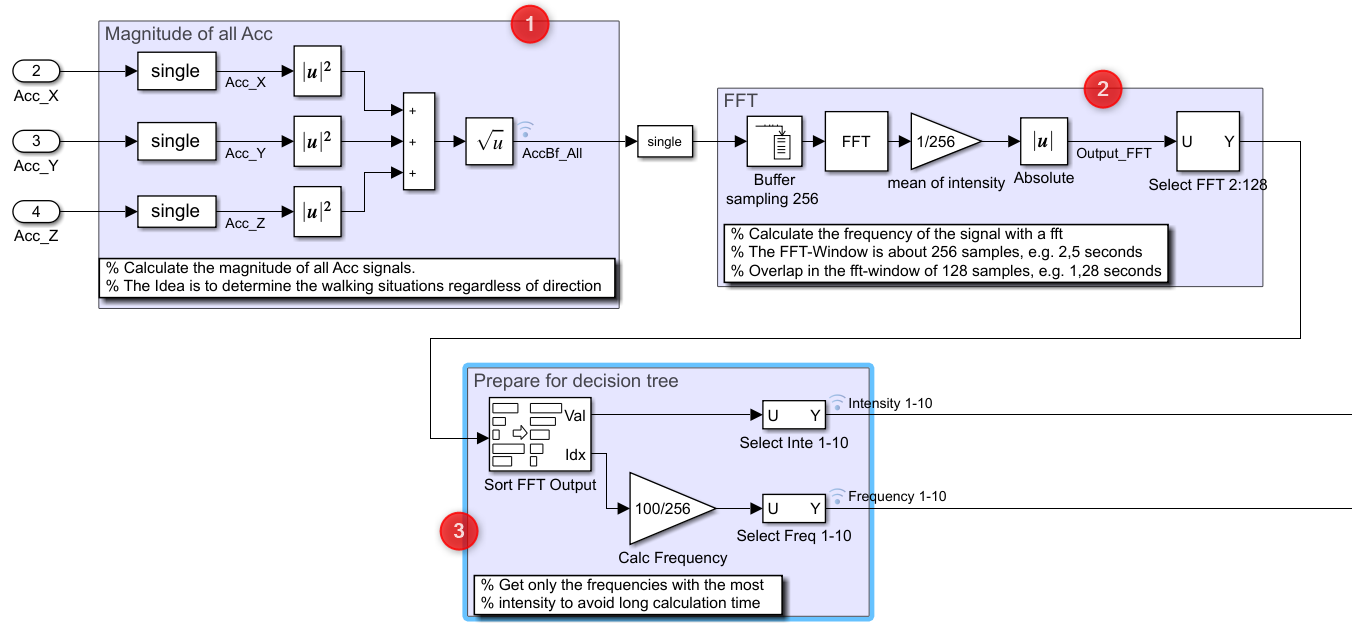
\includegraphics[width=\linewidth]{Bilder/Lauferkennung_Modell_1_1.png}
	\caption{Lauferkennung - Frequenzbasierte - FFT - Echtmodell}
	\label{fig:Lauferkennung_Freqbasiert_FFT_Echtmodell}
\end{figure}

Die vom dritten Teil ausgegangenen Daten werden zu einer Matlabdatei (\autoref{fig:getMotionClass_mFile}) geleitet, wo eine Entscheidung getroffen werden muss.
%
%Die AccBfX, AccBfY und AccBfZ sind die Ausgänge des Modells $CalibrationsMotorbike_V2$ und sie sind die Kalibrierte Signale.
%Diese Werte werden für die Berechnung der Betrag mit der Formel (**********************)
%%TODO: $AccBf_All=√(〖AccBfX〗^2+ 〖AccBfY〗^2+〖AccBfZ〗^2 )$ 
%verwendet (\autoref{fig:Lauferkennung_Freqbasiert_FFT_Spezifikationen})- Nummer 2). Das Ziel ist die Frequenzermittlung richtungsunabhängig zu stellen.
%Danach wurde eine FFT an der Variablen $AccBf_All$ durchgeführt, um die Frequenzen zu ermitteln (\autoref{fig:Lauferkennung_Freqbasiert_FFT}- Nummer 2).
%
%
%\begin{figure}[H]
%	\centering
%	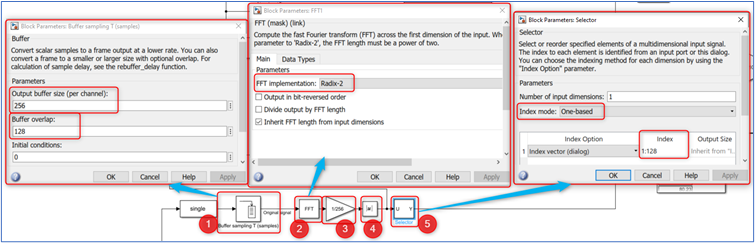
\includegraphics[width=\linewidth]{Bilder/Lauferkennung_Freqbasiert_FFT_Spezifikationen.png}
%	\caption{Testbeispiel - Frequenzbasierte Lauferkennung - FFT - Modell}
%	\label{fig:Lauferkennung_Freqbasiert_FFT_Spezifikationen}
%\end{figure}
%In der \autoref{fig:Lauferkennung_Freqbasiert_FFT_Spezifikationen} wird eine FFT durchgeführt. Die Einstellparameter jedes Element ist ersichtlich.

%1-	In der Buffer sind 256 Samples zu betrachten (d.h. ca. 2,5 Sekunden des Signals, da die Abtastrate der Sensor 100 Hz ist). Eine Überlappung von ca. 1 Sekunde wurde auch eingestellt, damit die Zwischen Frequenzen nicht übersehen werden.\\
%2-	Der FFT-Typ ist eine Radix-2.\\
%3-	Die Ausgabenwerte der FFT durch 265 dividieren. (warum?)\\ %TODO: warum 
%4-	Betrag des FFT-Ausgangs bilden (warum?)\\ %TODO: warum 
%5-	Da FFT ein gespiegelter Ausgang liefert wird nur die Hälfte der Matrix angenommen (1:128)\\
\subsubsection{Entscheidungskriterien - Matlabskript}
%
%
%
%
%
Die \autoref{fig:getMotionClass_mFile} zeigt die Matlab-Funktion, die die Entscheidung übers Laufen trifft. Die Eingänge der Funktion sind die zehn Frequenzen mit den höchsten zehn Intensitäten sowie die aktuelle Geschwindigkeit. Die durch die Funktion letzte erkannte Aktivität sowie deren Zeitpunkt werden auch in die Funktion geleitet. Nach dem Durchlauf liefert die Matlab-Funktion eine Id-Zahl, die eine Aktivität entspricht. Der Aktivität-ID-Zusammenhang ist in der \autoref{tab:MotionClass} abgebildet.

\begin{figure}[H]
	\centering
	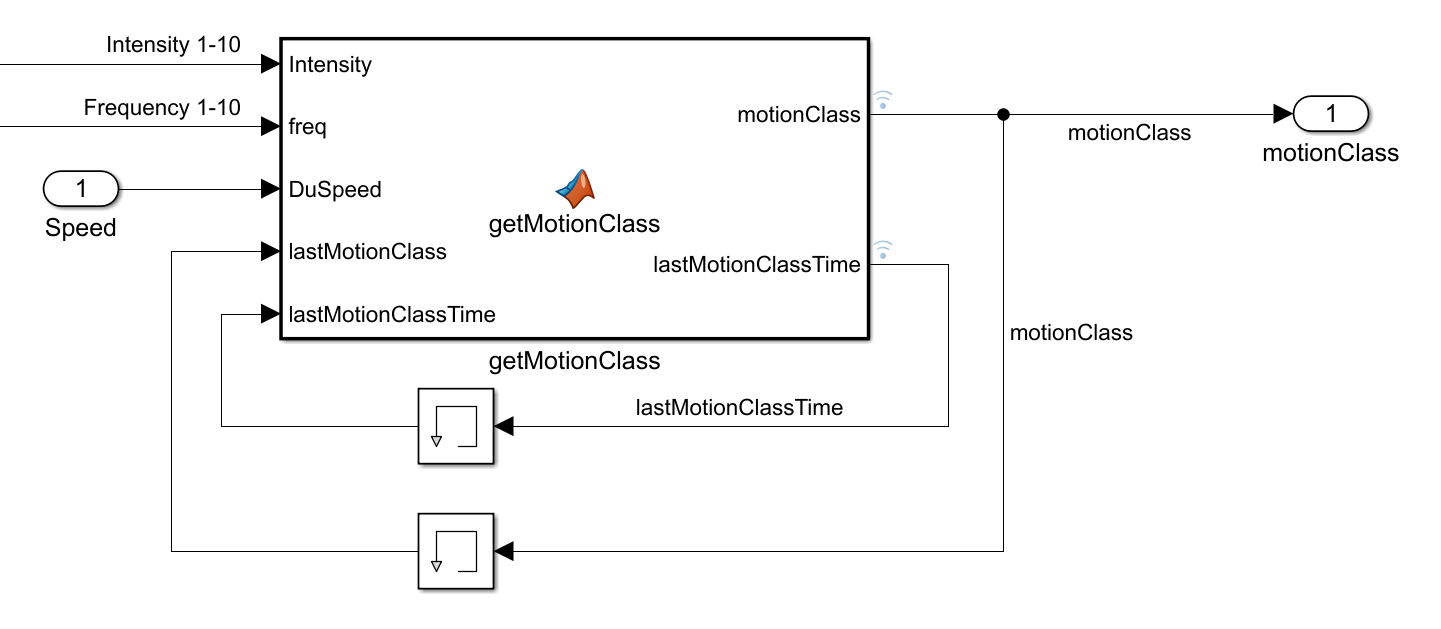
\includegraphics[width=\linewidth]{Bilder/getMotionClass_mFile.png}
	\caption{Ein- und Ausgänge des Entscheidungsskripts}
	\label{fig:getMotionClass_mFile}
\end{figure}

\begin{table}[H]
	\caption{Ausgangsmöglichkeiten der Entscheidungsfunktion} 
	\centering
	\begin{tabular}{|l|l|}%{|p{3.2cm}|>{\centering\arraybackslash}p{3.3cm}|>{\centering\arraybackslash}p{3.3cm}|>{\centering\arraybackslash}p{3.3cm}|}
			\hline
			\textbf{ID} & \textbf{Aktivität} \\
			\hline
			-1 & Konflikt/Fehler \\
			\hline
			0 & Keine Bewegung \\
			\hline
			1 & Laufen \\
			\hline
			2 & Fahren \\
			\hline
		\end{tabular}
	\label{tab:MotionClass}
\end{table}

\begin{figure}[H]
	\centering
	\includegraphics[width=\linewidth]{Bilder/Lauferkennung_FFT_Ablaufschema_mFile.jpg}
	\caption{Entscheidungsbaum des Laufens}
	\label{fig:Lauferkennung_FFT_Entscheidungsbaum_mFile}
\end{figure}

Die \autoref{fig:Lauferkennung_FFT_Entscheidungsbaum_mFile} zeigt das einfache Entscheidungsbaum, wonach eine Lauferkennung erfolgt wird. Die Entscheidung erfolgt in einer Matlab-Funktion innerhalb vom Simulink-Modell (siehe \autoref{Anh:Entscheidungsfunktion}).

Die drei Hauptkriterien sind die Frequenz mit ihrer Intensität sowie die gemessene Geschwindigkeit. Wenn die Intensität einen Zulässigen Wert hat, wird die dazu gehörige Frequenz berücksichtigt und danach die gelieferte Aussage mit der Geschwindigkeit nachgeprüft.
In dem Entscheidungsbaum sind vier Klassen definiert.
\begin{itemize}
	\item Stehen bzw. keine Bewegung
	\item Laufen
	\item Fahren
	\item Konflikt: Wenn die Entscheidungskriterien (Frequenz und Geschwindigkeit) verschiedene Aussagen liefern
\end{itemize}
Der Entscheidungsbaum fängt bei der Intensität an. Wenn die größte Intensität kleiner als der Schwellwert ($100$) ist, kann die dazugehörige Frequenz für die Entscheidung nicht vertrauend sein und werden die vier nachfolgenden Intensität untersucht. Sollte immer noch keine zulässige Intensität ergeben, wird sofort nach Geschwindigkeit geschaut und diese für die Entscheidung verwendet.

Z.B. Bei einer Geschwindigkeit von $30$ km/h ist von einer Fahr auszugehen und bei $3$ km/h ist das Laufen die richtige Entscheidung.

Kommt eine zulässige Intensität vor, wird die dazugehörige Frequenz berücksichtigt. Eine Frequenz unter $2$ Hz bedeutet 'laufen' und über $7$ Hz entspricht 'fahren'. Es wird danach mit der Geschwindigkeit nachgeprüft. Eine Geschwindigkeit von über $7$ km/h bedeutet auf jeden Fall 'Fahren' und darunter 'laufen'.
Wenn die Frequenz- und die Geschwindigkeitsüberprüfung verschiedene Aussagen zurückgeben, ist von einem 'Konflikt' auszugehen. In diesem Fall werden die vier nachfolgenden Frequenzen überprüft.


\subsubsection{Testbeispiel}
Die Signale in der \autoref{fig:AbschnitteBeispielsignal} sind aus einem Echtsignal ausgeschnitten, in dem der Fahrer nach einer Fahrt gelaufen ist. Das Fahren ist in der \autoref{fig:AccZ_Driving_8Sec} sowei das Laufen in der \autoref{fig:AccZ_Walking_8Sec} abgebildet.

Das Lauferkennung-Modell wurde mit dem entsprechenden Signal getestet. Das Modell hatte die richtigen Frequenzen erkannt.
Für das erste Teilsignal aus der \autoref{fig:AccZ_Driving_8Sec} hat eine Frequenz von durchschnittlich $20$ Hz geliefert. Das Teilsignal aus der \autoref{fig:AccZ_Walking_8Sec} hat eine Frequenz von etwa $1.8$ Hz. Die Frequenzermittlung der Lauferkennung war sehr nah zur Realität.
Nachdem die Frequenzen ermittelt wurden, sind diese ins Entscheidungsskript geleitet. Das Skript entscheidet dann mit einer Geschwindigkeitsprüfung, welche Aktivität (Fahren oder Laufen) durchgeführt wurde.


\begin{figure}[H]
	\centering
	\begin{subfigure}{\textwidth}
		\centering
		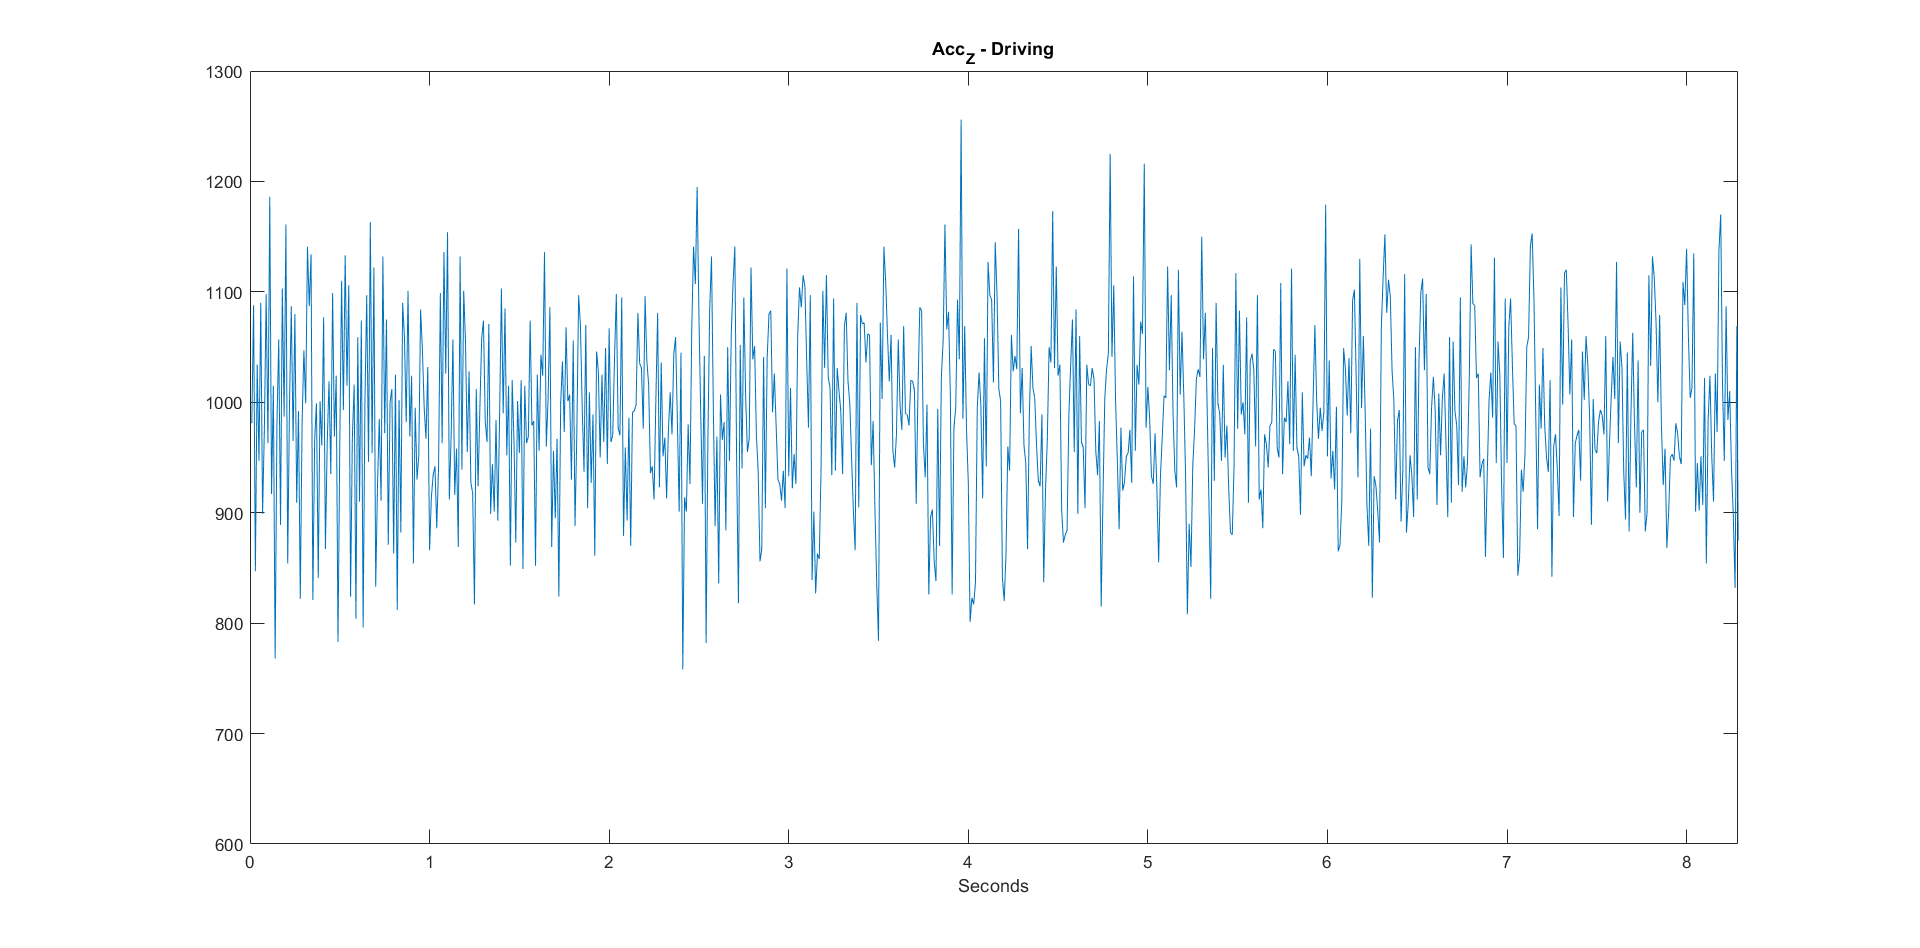
\includegraphics[width=\textwidth]{Bilder/AccZ_Driving_8Sec.png}
		\caption{Beispielsignal - Laufen}
		\label{fig:AccZ_Driving_8Sec}
	\end{subfigure}
	\hfill
	\begin{subfigure}{\textwidth}
		\centering
		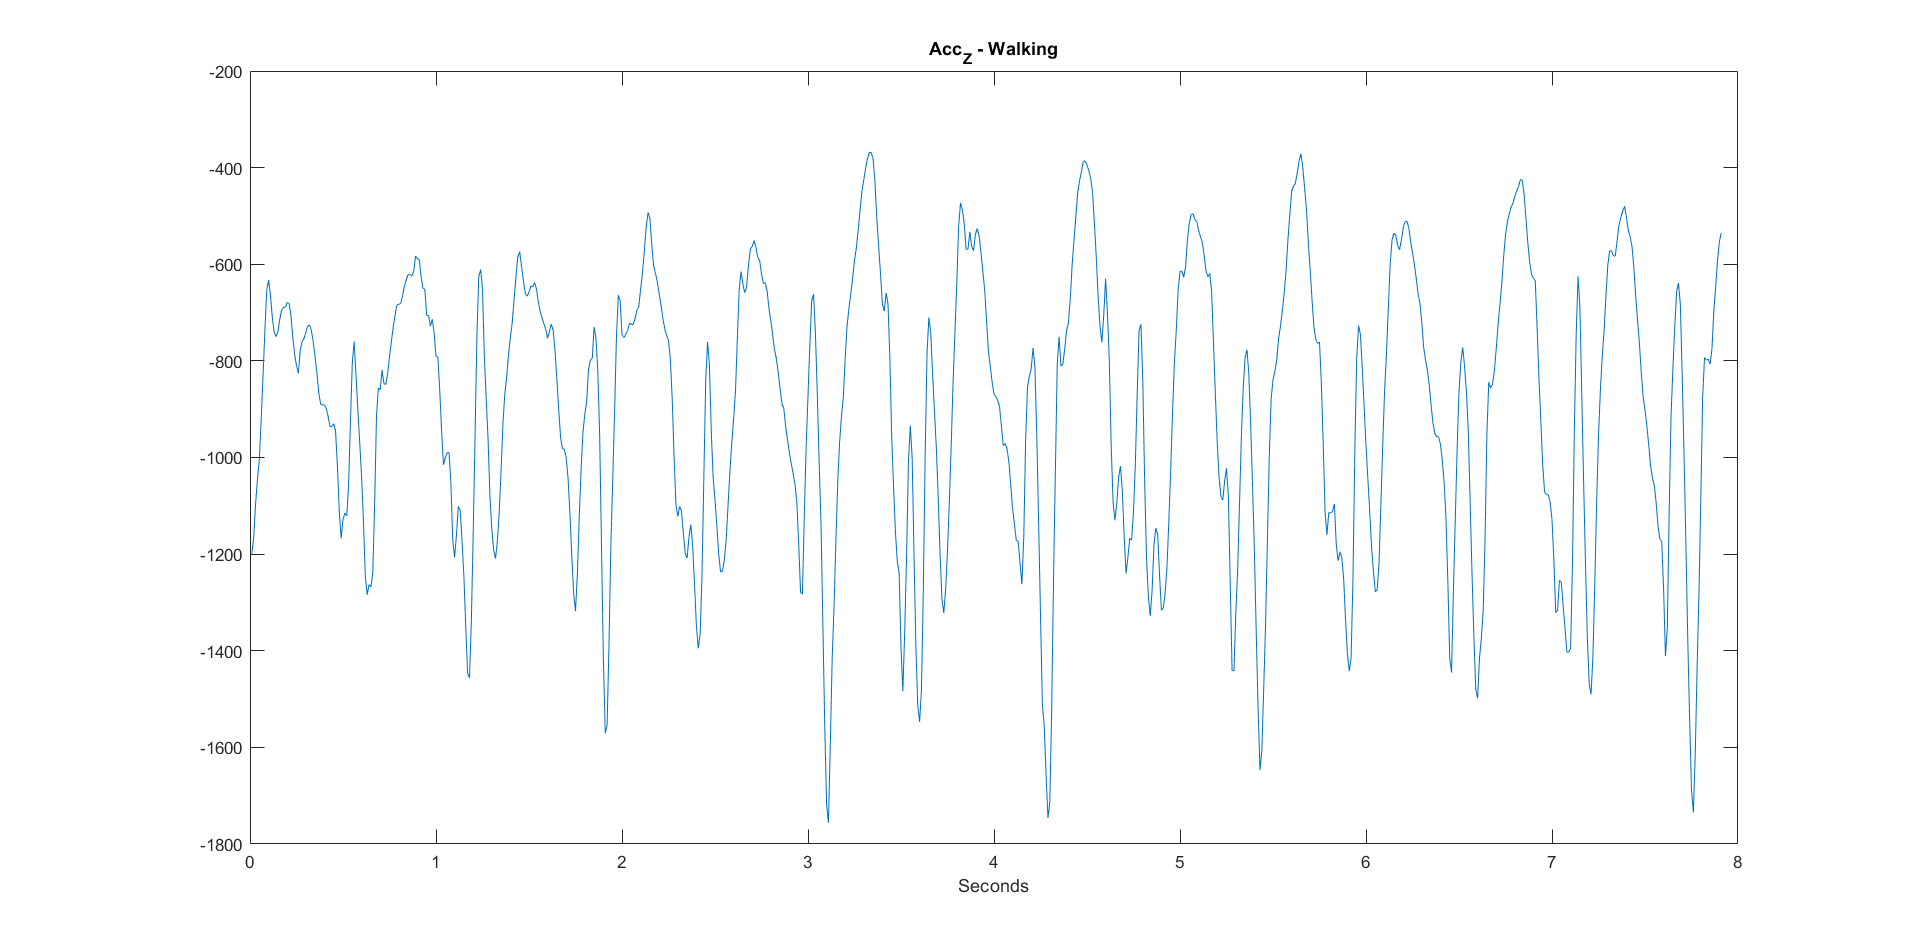
\includegraphics[width=\textwidth]{Bilder/AccZ_Walking_8Sec.png}
		\caption{Beispielsignal - Fahren}
		\label{fig:AccZ_Walking_8Sec}
	\end{subfigure}
	\caption{Abgeschnittene Teile eines Beispielsignals}
	\label{fig:AbschnitteBeispielsignal}
\end{figure}



%Mögliche Konflikte: ID = 2488; CrashNoPSAP;\\
%
%\begin{figure}[H]
%	\centering
%	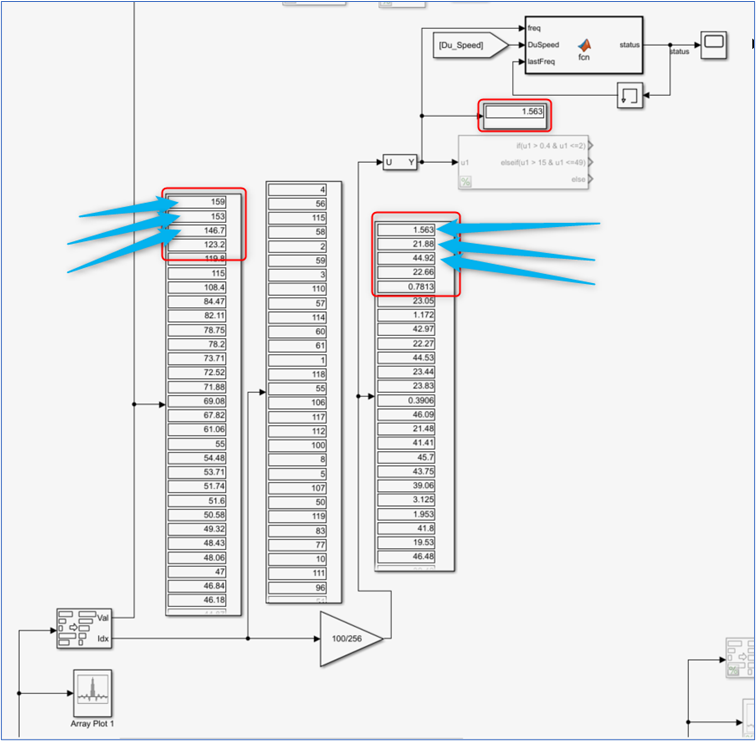
\includegraphics[width=\linewidth]{Bilder/Lauferkennung_Freqbasiert_Ausgangsbeispiel.png}
%	\caption{Testbeispiel - Frequenzbasierte Lauferkennung - Ausgangsbeispiel - ID 2488}
%	\label{fig:Lauferkennung_Freqbasiert_Ausgangsbeispiel_ID2488}
%\end{figure}
%Da hier (\autoref{fig:Lauferkennung_Freqbasiert_Ausgangsbeispiel_ID2488} und \autoref{fig:Lauferkennung_Freqbasiert_Ausgangsbeispiel_ID2488_Scope}) die maximale Intensität der Frequenz 1,5, wird diese als das Maximum übernommen und weiterbearbeitet. Die nächste größte Intensität liegt sehr nah dazu und hat die Frequenz 21,88 Hz, was eigentlich richtiger ist.
%
%\begin{figure}[H]
%	\centering
%	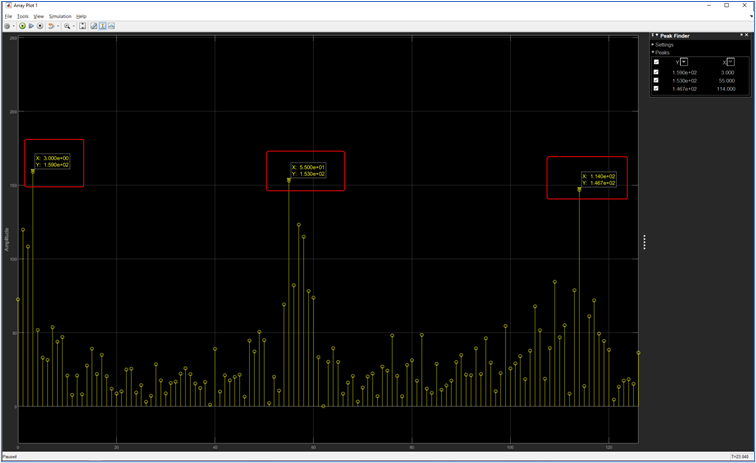
\includegraphics[width=\linewidth]{Bilder/Lauferkennung_Freqbasiert_Ausgangsbeispiel_ID2488_Scope.png}
%	\caption{Testbeispiel - Frequenzbasierte Lauferkennung - Ausgangsbeispiel - ID 2488 - Scope}
%	\label{fig:Lauferkennung_Freqbasiert_Ausgangsbeispiel_ID2488_Scope}
%\end{figure}




\subsubsection{Sinnvolle Werte auswählen}
Nachdem das Testmodell gute Ergebnisse geliefert hatte, sollen die Schwellwerte diskutiert werden.
\begin{itemize}
	\item \textbf{Intensität:} Der Entscheidungsbaum sucht nach einer Intensität von über 100, damit die dazugehörige Frequenz vertrauend zur Entscheidung verwendet wird. Nach mehreren Testungen wurde eine Intensität von 100 ausgewählt. Ein niedriger Intensitätswert führt zu einer möglichen falschen Entscheidung, da die Rauschen bzw. die kleinen Frequenzen aus dem Frequenzbereich fälschlicherweise in das Entscheidungsskript eingeleitet wurde.
	\item \textbf{Frequenzbereich:} das entspricht der Frequenzbereiche vom Laufen und vom Fahren.
	\item \textbf{Geschwindigkeit:} In dem Skript ist ein Wert von $7$ km/h als Schwellwert zwischen Fahren und Laufen ausgewählt. Der Wert ist in der Straßenverkehrsordnung als Schrittgeschwindigkeit anerkannt\citep{Bussgeldkataloge2022}. Erfahrungsmäßig läuft der Mensch in einer Geschwindigkeit zwischen $5$ und $10$ km/h.
\end{itemize}



\section{Auf- und Absteigen} \label{sec:AufAbsteigen} %TODO: Ausführlicher beschreiben. Mit Bilder.

Beim Auf- und Absteigen gibt's starke Winkeländerung im Raum (3D). Wenn einen GH erkannt wird, sollte einen Alarmauslösung ergeben. Ohne GH sollte der Fall nicht als Unfall erkannt.



\section{An Ampel stehen und Fuß runter} \label{sec:AmpelStehen} %TODO: Ausführlicher beschreiben. Mit Bilder
In diesem Abschnitt wird ein Szenario aus der Tabelle analysiert, in dem der Fahrer während einer Fahrt an eine Ampel für kurze Zeit anhält und sein Fuß runter setzt. In diesem Fall ist das Smartphone in der Hosentasche der bewegenden Bein.
Die Annahme, dass in so einem Fall im Pocket-Mode einen Falschen Alarm ausgelöst werden könnte. Der Grund ist die Winkeländerung von ca. 90\degree zwischen den zwei Positionen, was das Modell 'TipOver' aktiviert und zu einer Alarmauslösung führt.

Die erste Position ist das Bein während einer Fahrt mit der horizontalen Beinstellung. Wenn der Fuß am Boden ist, steht das Bein einer vertikalen Postion.

.\\

- Signalbeispiel mit Phasenmarkungen (Horizontal und Vertikal)

.\\


Nach dem Testen: Keine falsche Alarmauslösungen. Grund ist, dass die Winkeländerung nicht 90 grad beträgt sondern nur ca. 20-30 grad (\autoref{fig:MotorbikeDrivingStanding}). Die Person hat sein Bein beim Sitzen nicht genau horizontal sondern leicht nach Unten geneigt. Und wenn der Fahrer sein Fuß runter setzt, ist diese auch nicht genau vertikal sondern bisschen gebogen mit einem Winkel von ca. 10-20 Grad zum Vertikallinie. D.h. die Winkeländerung nicht 90 Grad ist.

\begin{figure}[H]
	\centering
	\begin{subfigure}{\textwidth}
		\centering
		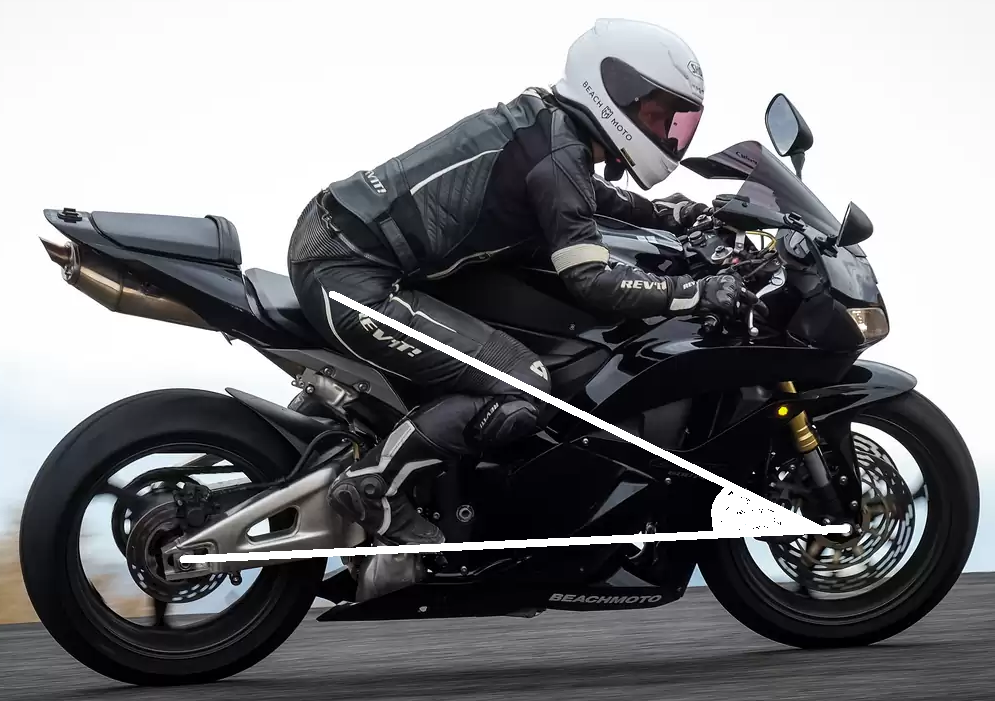
\includegraphics[width=0.5\textwidth]{Bilder/MotorbikeDriving2.png}
		\caption{Beinposition während einer Fahrt}
		\label{fig:MotorbikeDriving}
	\end{subfigure}
	\hfill
	\begin{subfigure}{\textwidth}
		\centering
		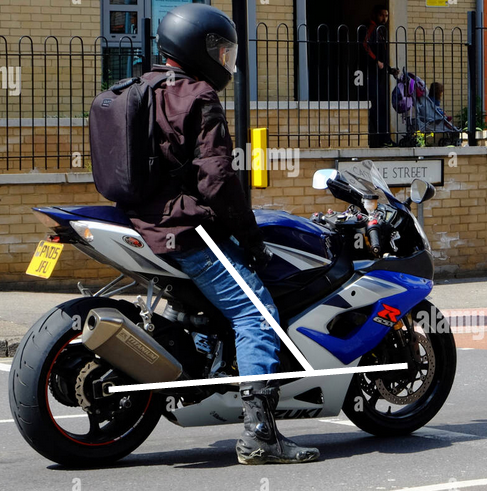
\includegraphics[width=0.5\textwidth]{Bilder/MotorbikeStanding2.png}
		\caption{Beinposition Beim Stehen}
		\label{fig:MotorbikeStanding2}
	\end{subfigure}
	\caption{Beinpositionen während einer Fahrt und gestreckt}
	\label{fig:MotorbikeDrivingStanding}
\end{figure}


\section{Verifikation des Algorithmus'}
% Aufgrund der Verifizierung des Algorithmus werden im Folgenden statistische Zahlen über Fahrradunfälle weltweit sowie in Deutschland dargestellt. Danach wird eine statistische Fallzahlabschätzung durchgeführt, um die notwendige Anzahl der Versuche zu ermitteln. Eine Versuchsplannung wird anhand der Ergebnisse der Versuche durchgeführt, die bereits vor der eigentlichen Verifizierung durchgeführt wurden. 
%
%
%


\subsection{Groundtruth-Daten sammeln, Tatsächliche Aktivitätsdaten}

Die Lauferkennung ergibt die Ausgabe (Fahren oder Laufen) und soll demnächst umfangreich getestet werden. Für die Testung muss der tatsächliche Verlauf einer Fahrt bekannt gegeben werden. Zu diesem Zweck wurden alte Crashtests mit Videos optisch manuell mithilfe eines intern entwickelten LabVIEW-Tool ausgewertet werden. Die Crashtests wurden mit mehreren am Motorrad befestigten Smartphones. Verschiedene Unfallszenarien wurden geprüft, wie z.B. gegen die Wand fahren oder während der Fahrt an einer Kurve rutschen. Diese Crashtests wurden mit Videos aufgenommen, die nur einen kleinen Teil der aufgezeichneten Signal abgedeckt haben. Damit die Videos dem richtigen Signalteil zugeordnet werden können, ist eine Synchronisierung zwischen dem Signal und dem dazugehörigen Video erforderlich. 

Mit dem internen Tool kann der Benutzer die Video-Signal-Synchronisierung unkompliziert erfolgen. Danach können bestimmte Labels (z.B. Fahren oder Stehen) für die entsprechenden Zeitfenster schnell und einfach eingegeben werden. Am Ende wird eine Tabelle exportiert, welche die gleiche originalen Daten sowie eine neue zusätzliche Spalte mit den Label-Ids der Aktivitäten beinhaltet.
Diese Tabelle kann mit den Ergebnissen der Lauferkennung verglichen werden.

Die erwähnte Labels muss der Benutzer vorhin definieren ins Tool einladen. In der \autoref{fig:TabCalimotoLabelsID} ist die Tabelle der definierten Labels sichtbar. Die Tabelle hat sieben verschiedene Klassen, die sich im Tool mit den F-Tasten einfach eingeben lassen. 'Undefined' entspricht unbekannte Eingabe, wenn das Motorrad nicht im Video sichtbar ist. 'Post-Crash' repräsentiert der Fall, wenn das Motorrad nach einem Sturz weiter rollt oder bis zu Ruhestand bewegt.
 
In der \autoref{fig:Exporttabelle_Davilt} ist ein verkürztes Beispiel der exportierten Tabelle, in der die neue Spalte 'GroundTruthId' sichtbar ist.
\begin{figure}[H]
	\centering
	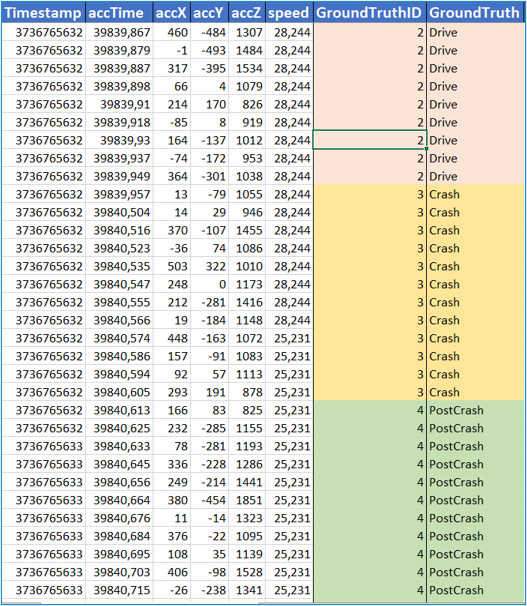
\includegraphics[width=\linewidth]{Bilder/Exporttabelle_Davilt.png}
	\caption{Beispiel der exportierten Tabelle mit der neuen Spalte}
	\label{fig:Exporttabelle_Davilt}
\end{figure}

\begin{figure}[H]
	\centering
	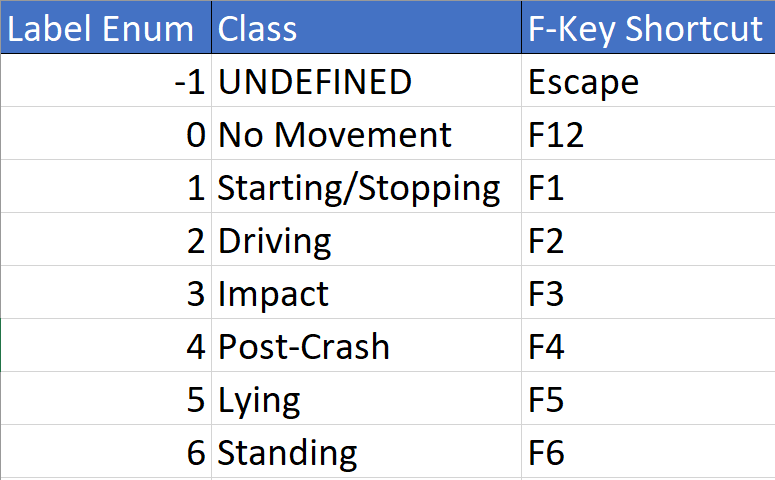
\includegraphics[width=0.6\linewidth]{Bilder/TabCalimotoLabelsID.png}
	\caption{Die definierte Labels}
	\label{fig:TabCalimotoLabelsID}
\end{figure}



- Videos mit den Daten synchronisieren (Das Tool erläutern? oder vllt. nur erwähnen?)\\
- Groundtruth labels nachdenken und erläutern\\
- Videos labeln\\









%\begin{table}\caption{Statistische Zahlen über Unfälle in Deutschland \cite{Verkehrsunfaelle_Fahrrad2017}} 
%	\centering
%	\begin{tabular}{|p{3.2cm}|>{\centering\arraybackslash}p{3.3cm}|>{\centering\arraybackslash}p{3.3cm}|>{\centering\arraybackslash}p{3.3cm}|}
	%		\hline
	%		\textbf{Jahr} & \textbf{Unfälle} & \textbf{Verunglückte} & \textbf{Getötete} \\
	%		\hline
	%		2000 & 382.949 & 511.577 & 7.503 \\
	%		\hline
	%		2005 & 336.619 & 438.804 & 5.361 \\
	%		\hline
	%		2010 & 288.297 & 374.818 & 3.648 \\
	%		\hline
	%		2014 & 302.435 & 392.912 & 3.377 \\
	%		\hline
	%		2015 & 305.659 & 396.891 & 3.459 \\
	%		\hline
	%		2016 & 308.145 & 399.872 & 3.206 \\
	%		\hline
	%		2017 & 302.656 & 393.492 & 3.180 \\
	%		\hline
	%	\end{tabular}
%	\label{tab:UnfallImJahren}
%\end{table}







